% Hai nghiên cứu, estimator và phạm vi bằng chứng được giữ riêng.
\chapter{Experiments and Discussion}\label{s:016253c474e8e6bb}
\section{Studies and evidence scope}\label{s:26fcfd1c2d723181}
The component study compares Full/Base and numerical controls, with
separate upstream and factorial/placebo panels. The historical-context
study compares eight roles conditional on one shared upstream realization
per point. They share a sampled market schedule but have separate
responses, protocol histories and estimators. Full is not a reused Native
response, and Base is not Common. Both studies are historical exploratory
assessments, with no new inference or retraining for this manuscript.

The component main has 204 Decision outputs. Its nine-unit, three-run
upstream panel has 54 cells, including 18 reused main outputs; the separate
five-branch factorial panel has 135 outputs. There are therefore 375
distinct executions, not independent samples obtained by adding all cells.
Context has $102\times3\times8=2,448$ slots: 1,290 raw Decision responses
and 1,158 no-request bypasses. Neither slots, HTTP attempts nor repeated
responses are new market observations. The six folds were already exposed;
the component queue freeze occurred after inference began. Immutable
hosted-weight revisions are unavailable. Artifact integrity and offline
replay do not establish prospective or whole-system causal validity.

\section{Data, partitions and coverage}\label{s:8be41ee200674674}
The purposive sample is FPT, CMG, VCB, MBB, MWG, VNM, BHN, HVN and VJC.
Table~\ref{tab:schedule} specifies twelve selected dates, not a continuous
daily backtest across 2023–2026. The 102 eligible points form 51 separate
stock--fold accounts, with 25 UP/77 DOWN labels. BHN supplies only the
last three folds: a contradictory 13 September 2022 candle is retained
in raw evidence but its prefix (673 rows) is excluded; the valid suffix
starts 14 September. Six absent market cells are structural exclusions,
not failed or losing forecasts.

\begin{table}[htbp]\centering\small\setstretch{1.05}
\caption{Shared sampled schedule. Each stock/fold has two endpoints;
accounts are counted per method/repeat.}\label{tab:schedule}
\begin{tabular}{@{}l llrr@{}}\toprule
Fold & First cutoff & Second cutoff & Points & Accounts\\\midrule
2023 H2 & 2023-07-03 & 2023-09-22 &16&8\\
2024 H2 & 2024-07-01 & 2024-09-20 &16&8\\
2025 H1 & 2025-01-02 & 2025-03-31 &16&8\\
2025 Q4 & 2025-10-01 & 2025-12-19 &18&9\\
2026 Q2 & 2026-04-01 & 2026-06-24 &18&9\\
2026 Q3 & 2026-07-01 & 2026-09-23 &18&9\\\midrule
Total & \multicolumn{2}{l}{Nine stocks; twelve dates} &102&51\\\bottomrule
\end{tabular}\end{table}

Pinned vendor/cache material does not independently authenticate
contemporaneous data availability. The reconstructed VCI/vnstock daily
retrieval is explicitly a new retrieval, not an authenticated original
run snapshot; action/dividend adjustment evidence is incomplete.
Sentiment is unavailable at 79/102 context points. The 852-row signal
bank covers four stocks and 48 query points; the remaining 54 retain
Common fallback. Numerical task context is separately frozen per fold,
with reserved evaluation IDs excluded. Missing support/news stays in
primary results.

Component controls use 51 chronological purged scopes (32–318 train and
18–21 validation cycles); all 51 recorded purge checks pass. Context
instead has nine unique fixed-per-stock Common selectors, referenced by
51 bindings. Eight non-BHN selectors use train decisions 14 April
2021–30 September 2022 (123 cycles) and validation 6 October 2022–27 June
2023 (54–60 common cycles). BHN uses 20 December 2023–26 December 2024
train (85) and 2 January–25 September 2025 validation (56). Labels mature
before the next split. The MT teacher/scaler train through 2020; 2021
selects the student and 2022 assesses it, as Chapter 4 specifies. These
resource schedules and disclosed amendments do not create fresh holdouts.

\section{Recorded configuration and paired protocol}\label{s:21f290190e1fcedc}
Both recorded environments use Python 3.13.5, NumPy 2.1.2, pandas 2.3.3,
SciPy 1.16.1, scikit-learn 1.7.2 and TA-Lib .6.8. Hosted vision alias is
\texttt{qwen/qwen3.8-27b}; Decision alias is \texttt{openai/gpt-oss-20b}.
Declared temperature is zero; archived wire metadata records $10^{-8}$.
Component vision/Decision output caps are 1,024/2,048 tokens; context caps
are 960/960. Original prompts are Vietnamese. These aliases/options and
source/resource pins identify the historical configuration, not current
live defaults or immutable hosted weights.

Upstream is generated once per point and deep-copied across methods.
Context repeats only Decision three times, with same-repeat dependency
reuse and durable outcome barriers. Component metadata retain forty
paired order mismatches and nine groups spanning execution epochs;
perfect counterbalancing is not established. Context's HTTP ledger has
1,702 attempts and retains 15 retired records, separately from active
responses. Coverage and failures cannot be recoded to reach planned slots.

\section{Comparators and interventions}\label{s:351598650d1ea43f}
Component main controls are CASH, train-majority (strictly more than half
train labels UP), always-LONG cycles, positive 20-session momentum,
price logistic, matched numerical-input logistic and oriented factor
vote. Logistic validation chooses $C\in\{.01,.1,1,10\}$ and thresholds in
order $(.5,.4,.6)$ by BA, retaining first ties; train imputation/missing
indicators/scaling precede selected train+validation refit (lbfgs,
3,000-iteration ceiling). Continuous holding is a separate price-only
financial reference, not always-LONG sampled cycles.

The factorial panel uses B/A/S/AS/P for neither/alpha/sentiment/both/
sentiment-plus-past-donor-alpha values on nine units and three executions.
Its full-value prompts differ from main compact prompts. A separate
23-strategy numerical experiment retains fixed five, train-ranked five,
the same five without sign flip and all twenty random-five trials. It
uses no hosted calls and is not an isolated LLM-selector ablation.
Context compares five extensions (v1/C2/A/B/MT) against \emph{both} Native
and Common, with separate Common--Anchor--MT bridges; controls are CASH
and always-LONG cycles. Missing matched context ablations remain missing.

\section{Metrics and descriptive uncertainty}\label{s:ef6038a5b0f5c76d}
Final LONG predicts UP; CASH predicts DOWN. With confusion counts over
the 25/77 class support, BA and MCC are
\begin{align}
BA&=\tfrac12\left(\frac{TP}{TP+FN}+\frac{TN}{TN+FP}\right),\\
MCC&=\frac{TP\,TN-FP\,FN}{\sqrt{(TP+FP)(TP+FN)(TN+FP)(TN+FN)}}.
\end{align}
Accuracy is $(TP+TN)/N$; LONG rate $(TP+FP)/N$. Macro-F1 averages the
class F1 scores, not stocks. Undefined denominators remain NA with reasons;
constant predictions can have defined BA but undefined MCC. Context pools
confusion over points within each repeat, then averages the three scores.
Percentages and percentage-point (pp) differences are distinguished.

Each VND 50-million reference account compounds nonoverlapping cycle
payoffs from Equation~\ref{eq:label}, using fractional all-in LONG/CASH:
\begin{equation}
R_{qmr}=\prod_{i\in q}(1+z_{imr})-1,\qquad
\bar R_m^{(\%)}=\frac{100}{51}\sum_{q=1}^{51}\frac13\sum_{r=0}^2R_{qmr}.
\end{equation}
Component main averages its 51 accounts without Decision repeats. The
separate numerical headline instead averages nine stock-level accounts;
it is not that 51-account estimator. Positive-magnitude EOD drawdown is
$100\max_d(1-V_d/\max_{u\le d}V_u)$. Account averages are not a shared-capital
portfolio. Component daily Sharpe uses population SD and nominal
$\sqrt{252}$; its legacy Sortino uses SD of negative returns. Context
uses unannualized cycle mean/sample-SD and downside RMS over all cycles,
including zero; annualized fields remain null. Ratios across these
conventions must not be ranked interchangeably.

Component main uses 10,000 paired whole-block bootstrap draws, seed
20261102; class-deficient draws remain undefined. Its factorial seven-BA
family uses an unstandardized centered maximum-deviation envelope on
6,986 jointly finite draws (3,014 undefined). Numerical diagnostics use
10,000 block draws, seed 0, 64 block-sign assignments and Holm over all
23 BA contrasts, under unverified symmetry assumptions.

Context's full family has twenty cells: five extensions, two baselines
and return/BA endpoints. Circular length-two blocks resample six fold
positions, preserving stocks, methods/repeats and account resets (10,000
draws, PCG64 seed 20261110). With paired estimates $\hat\delta_j$ and
bootstrap SD $s_j$, its descriptive band is
\begin{equation}
M_b=\max_j\frac{|\delta^*_{bj}-\hat\delta_j|}{s_j},\quad
c=Q_{.95}^{higher}(M),\quad [\hat\delta_j-cs_j,\hat\delta_j+cs_j].
\end{equation}
The whole family needs at least 9,500 jointly finite draws, finite point
estimates and nonzero finite SD in every cell; otherwise bands are null.
The saved primary family has 10,000 finite draws. Length-one/three,
CORE4 and leave-one-fold/stock analyses are sensitivities, not independent
confirmation. Six exposed clusters do not establish calibrated coverage,
power, significance or causal superiority. No bootstrap was regenerated.

\section{Component-study results}\label{s:1859e39b7acb256f}

\hyperref[s:76f293631b51a105]{Appendix D.1--D.2} retains the extended Full/Base group confusion rows and every saved execution-level row of the two smaller panels.

The full component system improves some classification measures over Base
on the recorded main sample, but its mean account return is slightly
lower. Price-only logistic regression has higher pooled BA than Full,
and CASH has a higher mean return than every active main comparator.
The small upstream and factorial panels give different rankings. Together,
these observations support a conditional description of the system's
behavior, rather than a general advantage from adding alpha and sentiment.
All results below use the locked component collection introduced in
Section 5.1. They are separate from the historical-context results in
Section 5.7.

\subsection{Main comparison and economic outcomes}\label{s:2656a895d58787ac}

\textbf{Table B05a. Main component comparison.} Classification uses the same
102 points, with 25 UP and 77 DOWN labels, nine stocks, twelve dates and
six blocks. Each financial mean uses 51 separate stock--fold accounts.
Acc., BA and LONG rate are percentages; MCC and macro-F1 are unitless.
Returns and positive-magnitude EOD maximum drawdowns are percentages,
averaged equally across accounts under the fractional reference ledger.
The continuous-hold control has no pointwise classification output:
its classification entries are NA, while its recorded financial
support is 51 accounts. Display precision is three decimals; contrasts
use the saved unrounded values.\footnote{Main B05a/b cells: root exports ED32--ED34, classification support ED35; CL145--CL147 and ledger §10.7. Continuous hold retains zero classification units and 51 financial accounts. Original artifact values are retained at source precision; displayed rounding changes no estimator.}

\begin{landscape}
\begingroup
\fontsize{9}{11}\selectfont
\setstretch{1.05}
\setlength{\tabcolsep}{3pt}

\begin{longtable}[]{@{}
  >{\raggedright\arraybackslash}p{(\linewidth - 14\tabcolsep) * \real{0.1250}}
  >{\raggedright\arraybackslash}p{(\linewidth - 14\tabcolsep) * \real{0.1250}}
  >{\raggedright\arraybackslash}p{(\linewidth - 14\tabcolsep) * \real{0.1250}}
  >{\raggedright\arraybackslash}p{(\linewidth - 14\tabcolsep) * \real{0.1250}}
  >{\raggedright\arraybackslash}p{(\linewidth - 14\tabcolsep) * \real{0.1250}}
  >{\raggedright\arraybackslash}p{(\linewidth - 14\tabcolsep) * \real{0.1250}}
  >{\raggedright\arraybackslash}p{(\linewidth - 14\tabcolsep) * \real{0.1250}}
  >{\raggedright\arraybackslash}p{(\linewidth - 14\tabcolsep) * \real{0.1250}}@{}}
\caption{Table B05a. Main component comparison.}\label{tab:05_experiments:11}\tabularnewline
\toprule\noalign{}
Method
 & Acc. (\%)
 & BA (\%)
 & MCC
 & Macro-F1
 & LONG (\%)
 & Mean return (\%)
 & Mean MDD (\%)
 \\
\midrule\noalign{}
\endfirsthead
\toprule\noalign{}
Method
 & Acc. (\%)
 & BA (\%)
 & MCC
 & Macro-F1
 & LONG (\%)
 & Mean return (\%)
 & Mean MDD (\%)
 \\
\midrule\noalign{}
\endhead
\bottomrule\noalign{}
\endlastfoot
Full & 65.686 & 52.961 & 0.060 & 0.530 & 23.529 & -0.797 & 1.367 \\
Base & 60.784 & 49.714 & -0.005 & 0.496 & 28.431 & -0.750 & 1.453 \\
CASH & 75.490 & 50.000 & NA & 0.430 & 0.000 & 0.000 & 0.000 \\
Train-majority & 75.490 & 50.000 & NA & 0.430 & 0.000 & 0.000 & 0.000 \\
Always-LONG cycles & 24.510 & 50.000 & NA & 0.197 & 100.000 & -3.000 & 4.523 \\
Momentum 20 & 49.020 & 47.325 & -0.046 & 0.449 & 48.039 & -1.636 & 2.576 \\
Logistic price & 67.647 & 55.610 & 0.114 & 0.557 & 23.529 & -0.683 & 1.177 \\
Logistic matched inputs & 60.784 & 52.416 & 0.044 & 0.518 & 32.353 & -1.105 & 1.602 \\
Factor vote & 51.961 & 51.974 & 0.034 & 0.483 & 49.020 & -1.457 & 2.488 \\
Continuous hold (price only) & NA & NA & NA & NA & NA & -2.127 & 12.939 \\
\end{longtable}

\endgroup
\end{landscape}

Full's pooled BA is 52.961\%, compared with 49.714\% for Base: a difference
of \textbf{+3.247 percentage points (pp)}. Accuracy increases by 4.902 pp and
MCC moves from a small negative value to 0.060. This gain does not imply
strong UP detection. Table B05b shows that both methods identify only
7 of the 25 UP outcomes, giving UP recall of 28.000\%. Full has five fewer
false positives in aggregate, while retaining the same true-positive
count; this is an aggregate confusion comparison, not a claim that
exactly five individual actions changed.

\textbf{Table B05b. Full/Base confusion counts and recorded exposure.} TP/FN
refer to UP; TN/FP refer to DOWN. LONG/CASH counts sum to 102. Exposure
columns are means of the 51 account fractions over the ledger calendar,
including cash gaps; they are distinct from the fraction of scheduled
decisions classified LONG.\footnote{Main B05a/b cells: root exports ED32--ED34, classification support ED35; CL145--CL147 and ledger §10.7. Continuous hold retains zero classification units and 51 financial accounts. Original artifact values are retained at source precision; displayed rounding changes no estimator.}

\begin{landscape}
\begingroup
\fontsize{9}{11}\selectfont
\setstretch{1.05}
\setlength{\tabcolsep}{3pt}

\begin{longtable}[]{@{}
  >{\raggedright\arraybackslash}p{(\linewidth - 16\tabcolsep) * \real{0.1111}}
  >{\raggedright\arraybackslash}p{(\linewidth - 16\tabcolsep) * \real{0.1111}}
  >{\raggedright\arraybackslash}p{(\linewidth - 16\tabcolsep) * \real{0.1111}}
  >{\raggedright\arraybackslash}p{(\linewidth - 16\tabcolsep) * \real{0.1111}}
  >{\raggedright\arraybackslash}p{(\linewidth - 16\tabcolsep) * \real{0.1111}}
  >{\raggedright\arraybackslash}p{(\linewidth - 16\tabcolsep) * \real{0.1111}}
  >{\raggedright\arraybackslash}p{(\linewidth - 16\tabcolsep) * \real{0.1111}}
  >{\raggedright\arraybackslash}p{(\linewidth - 16\tabcolsep) * \real{0.1111}}
  >{\raggedright\arraybackslash}p{(\linewidth - 16\tabcolsep) * \real{0.1112}}@{}}
\caption{Table B05b. Full/Base confusion counts and recorded exposure.}\label{tab:05_experiments:12}\tabularnewline
\toprule\noalign{}
Method
 & TP
 & FN
 & TN
 & FP
 & LONG
 & CASH
 & Held sessions (\%)
 & Close exposure (\%)
 \\
\midrule\noalign{}
\endfirsthead
\toprule\noalign{}
Method
 & TP
 & FN
 & TN
 & FP
 & LONG
 & CASH
 & Held sessions (\%)
 & Close exposure (\%)
 \\
\midrule\noalign{}
\endhead
\bottomrule\noalign{}
\endlastfoot
Full & 7 & 18 & 60 & 17 & 24 & 78 & 2.353 & 1.569 \\
Base & 7 & 18 & 55 & 22 & 29 & 73 & 2.843 & 1.895 \\
\end{longtable}

\endgroup
\end{landscape}

The majority DOWN class explains why CASH and train-majority reach
75.490\% accuracy despite BA of 50.000\%, no UP detections and undefined
MCC. They retain their NA values rather than being assigned zero MCC.
Full's BA exceeds these constant controls by only 2.961 pp.~Logistic
price reaches BA of 55.610\% and MCC of 0.114, both above Full. The matched
input logistic control reaches BA of 52.416\%, slightly below Full, while
the factor vote reaches 51.974\%. These are observed rankings under their
recorded representations and fitting protocols, not evidence that all
comparators received identical information in identical form.

The saved six-block percentile interval for Full minus Base BA is
\textbf{{[}\ensuremath{-}1.176, 8.125{]} pp}, from 10,000 draws with no undefined draws. All
eight saved main BA intervals comparing Full with the other classification
methods include zero. As specified in Section 5.5, these are descriptive
historical block-bootstrap intervals, not evidence of confirmed
superiority or calibrated coverage.\footnote{ED28 \texttt{cohorts.\allowbreak{}all\_\allowbreak{}102.\allowbreak{}intervals}, eight contrasts, 10,000 draws each; CL145, ledger §10.7. The displayed Full/Base difference is direct arithmetic on ED33, not a new bootstrap.}

Full's mean net account return is \ensuremath{-}0.797\%, compared with \ensuremath{-}0.750\% for
Base. The unrounded difference is \textbf{\ensuremath{-}0.047 pp}, so the classification
improvement does not translate into a higher mean return. Full does have
lower average drawdown and lower held-session exposure than Base, but
both returns remain negative. Among active main comparators, logistic
price has the least negative mean return, \ensuremath{-}0.683\%; CASH and train-majority
remain at 0.000\%. Always-LONG cycles lose 3.000\% on average. The
continuous-hold result, \ensuremath{-}2.127\%, belongs to a different holding rule and
cannot be treated as an always-LONG classification strategy.

The divergence between BA and return is expected to be possible under
the estimators in Section 5.5: classification counts outcomes, whereas
account returns depend on the magnitude and sequence of selected net
cycles. Lower exposure can reduce losses and drawdown without establishing
a profitable signal. These account averages are neither an investable
multi-stock portfolio return nor an execution-certified performance
record.

\subsection{Stock and temporal-block patterns}\label{s:0892b467b27e8b87}

\textbf{Table B05c. Full/Base BA on every recorded stock and block.} Each row
uses its own shared Full/Base support; stock rows and block rows are two
overlapping partitions of the same 102 points. NA means that BA is
undefined because one outcome class is absent. The rows must not be
summed together or treated as independent replications.\footnote{ED35 \texttt{classification.\allowbreak{}csv}, \texttt{all\_\allowbreak{}102}/\texttt{symbol} and \texttt{block}, paired \texttt{AS}/\texttt{B} rows; ED36 retains equal-stock macro denominators; CL148, ledger §10.7. One-class rows remain visible as NA.}

\begingroup
\small
\setstretch{1.05}
\setlength{\tabcolsep}{3pt}

\begin{longtable}[]{@{}
  >{\raggedright\arraybackslash}p{(\linewidth - 8\tabcolsep) * \real{0.2000}}
  >{\raggedright\arraybackslash}p{(\linewidth - 8\tabcolsep) * \real{0.2000}}
  >{\raggedright\arraybackslash}p{(\linewidth - 8\tabcolsep) * \real{0.2000}}
  >{\raggedright\arraybackslash}p{(\linewidth - 8\tabcolsep) * \real{0.2000}}
  >{\raggedright\arraybackslash}p{(\linewidth - 8\tabcolsep) * \real{0.2000}}@{}}
\caption{Table B05c. Full/Base BA on every recorded stock and block.}\label{tab:05_experiments:13}\tabularnewline
\toprule\noalign{}
Group
 & Points
 & UP/\allowbreak{}DOWN
 & Full BA (\%)
 & Base BA (\%)
 \\
\midrule\noalign{}
\endfirsthead
\toprule\noalign{}
Group
 & Points
 & UP/\allowbreak{}DOWN
 & Full BA (\%)
 & Base BA (\%)
 \\
\midrule\noalign{}
\endhead
\bottomrule\noalign{}
\endlastfoot
symbol: BHN & 6 & 1/5 & 100.000 & 80.000 \\
symbol: CMG & 12 & 3/9 & 44.444 & 61.111 \\
symbol: FPT & 12 & 2/10 & 40.000 & 30.000 \\
symbol: HVN & 12 & 2/10 & 60.000 & 60.000 \\
symbol: MBB & 12 & 5/7 & 48.571 & 55.714 \\
symbol: MWG & 12 & 4/8 & 56.250 & 50.000 \\
symbol: VCB & 12 & 4/8 & 50.000 & 37.500 \\
symbol: VJC & 12 & 4/8 & 43.750 & 37.500 \\
symbol: VNM & 12 & 0/12 & NA & NA \\
block: b2023\_\allowbreak{}h2 & 16 & 3/13 & 38.462 & 34.615 \\
block: b2024\_\allowbreak{}h2 & 16 & 7/9 & 49.206 & 49.206 \\
block: b2025\_\allowbreak{}h1 & 16 & 0/16 & NA & NA \\
block: f2025\_\allowbreak{}q4 & 18 & 7/11 & 59.740 & 55.195 \\
block: f2026\_\allowbreak{}q2 & 18 & 6/12 & 45.833 & 45.833 \\
block: f2026\_\allowbreak{}q3 & 18 & 2/16 & 62.500 & 50.000 \\
\end{longtable}

\endgroup

The aggregate result is heterogeneous. Full has higher BA on five stocks,
lower BA on CMG and MBB, and the same BA on HVN. VNM has no UP outcome,
so its BA is undefined for both methods. BHN's apparently perfect Full
BA comes from only six observations with one UP outcome, over its shorter
admissible history. It therefore cannot support a broad stock-specific
performance claim. Full's BA is below 50\% on CMG, FPT, MBB and VJC.

Among the five blocks with defined BA, Full exceeds Base in three and
ties it in two. The remaining block, \texttt{b2025\_\allowbreak{}h1}, contains sixteen DOWN
outcomes and no UP outcomes. Full is itself below 50\% BA in three of the
five defined blocks. These small, uneven supports explain why pooled
and equal-stock summaries answer different questions. No stock or block
is removed from the primary result because its outcome is unfavorable
or its BA is undefined. Additional cohort and dependence sensitivities
belong to the later robustness analysis.

\subsection{Separate numerical factor controls}\label{s:b9245bd6063a38ed}

\textbf{Table B05d. Numerical five-factor controls.} Each strategy is evaluated
on the same 102 points with 25 UP and 77 DOWN outcomes. The 23 strategies
comprise three named rules and all twenty random-factor trials. The last
row reports the mean of the twenty trial metrics, not an ensemble's
actions. Unlike B05a, the return column is the saved mean of \textbf{nine
stock-level account returns}, not the mean of 51 stock--fold accounts;
its level should not be ranked directly against B05a.\footnote{ED24 \texttt{headline}, \texttt{random\_\allowbreak{}family}, \texttt{holm\_\allowbreak{}rejections}; ED25 \texttt{contrasts}, full family and draw metadata; CL149--CL150, ledger §10.7. This is the separate 23-rule numerical panel, not the factor-vote row of B05a.}

\begingroup
\small
\setstretch{1.05}
\setlength{\tabcolsep}{3pt}

\begin{longtable}[]{@{}
  >{\raggedright\arraybackslash}p{(\linewidth - 10\tabcolsep) * \real{0.1667}}
  >{\raggedright\arraybackslash}p{(\linewidth - 10\tabcolsep) * \real{0.1667}}
  >{\raggedright\arraybackslash}p{(\linewidth - 10\tabcolsep) * \real{0.1667}}
  >{\raggedright\arraybackslash}p{(\linewidth - 10\tabcolsep) * \real{0.1667}}
  >{\raggedright\arraybackslash}p{(\linewidth - 10\tabcolsep) * \real{0.1667}}
  >{\raggedright\arraybackslash}p{(\linewidth - 10\tabcolsep) * \real{0.1665}}@{}}
\caption{Table B05d. Numerical five-factor controls.}\label{tab:05_experiments:14}\tabularnewline
\toprule\noalign{}
Numerical strategy
 & Acc. (\%)
 & BA (\%)
 & MCC
 & LONG (\%)
 & Mean stock return (\%)
 \\
\midrule\noalign{}
\endfirsthead
\toprule\noalign{}
Numerical strategy
 & Acc. (\%)
 & BA (\%)
 & MCC
 & LONG (\%)
 & Mean stock return (\%)
 \\
\midrule\noalign{}
\endhead
\bottomrule\noalign{}
\endlastfoot
Fixed five & 49.020 & 39.221 & -0.193 & 36.275 & -8.653 \\
Train-ranked five & 62.745 & 55.065 & 0.093 & 32.353 & -5.648 \\
Same five, no sign flip & 50.980 & 48.623 & -0.024 & 46.078 & -7.608 \\
Random five (mean of 20) & 51.275 & 47.738 & -0.039 & 44.216 & -8.097 \\
\end{longtable}

\endgroup

Train-ranked factors improve pooled BA over the fixed set by 15.844 pp,
over the random-trial mean by 7.327 pp, and over the same selected IDs
without sign flipping by 6.442 pp.~Their mean stock return is nevertheless
negative at \ensuremath{-}5.648\%. All twenty random trials also have negative mean
stock returns. The saved random BA dispersion is 47.738\% \ensuremath{\pm} 5.377 pp
(mean \ensuremath{\pm} trial SD), with range {[}37.974\%, 57.169\%{]}; mean stock return is
\ensuremath{-}8.097\% \ensuremath{\pm} 1.404 pp, with range {[}\ensuremath{-}10.414\%, \ensuremath{-}5.537\%{]}. These are variations
across retained random factor sets, not confidence intervals over future
markets. No favorable seed is selected.

\textbf{Table B05e. Three declared numerical contrasts within the full family
of 23 diagnostics.} BA differences and saved percentile intervals are
in pp.~The exact two-sided diagnostics use all 64 block-sign assignments;
Holm adjustment uses all 23 contrasts, including the twenty individual
random-trial comparisons.\footnote{ED24 \texttt{headline}, \texttt{random\_\allowbreak{}family}, \texttt{holm\_\allowbreak{}rejections}; ED25 \texttt{contrasts}, full family and draw metadata; CL149--CL150, ledger §10.7. This is the separate 23-rule numerical panel, not the factor-vote row of B05a.}

\begingroup
\small
\setstretch{1.05}
\setlength{\tabcolsep}{3pt}

\begin{longtable}[]{@{}
  >{\raggedright\arraybackslash}p{(\linewidth - 8\tabcolsep) * \real{0.2000}}
  >{\raggedright\arraybackslash}p{(\linewidth - 8\tabcolsep) * \real{0.2000}}
  >{\raggedright\arraybackslash}p{(\linewidth - 8\tabcolsep) * \real{0.2000}}
  >{\raggedright\arraybackslash}p{(\linewidth - 8\tabcolsep) * \real{0.2000}}
  >{\raggedright\arraybackslash}p{(\linewidth - 8\tabcolsep) * \real{0.2000}}@{}}
\caption{Table B05e. Three declared numerical contrasts within the full family of 23 diagnostics.}\label{tab:05_experiments:15}\tabularnewline
\toprule\noalign{}
Recorded contrast
 & BA difference (pp)
 & Percentile interval (pp)
 & Exact p
 & Holm p (23)
 \\
\midrule\noalign{}
\endfirsthead
\toprule\noalign{}
Recorded contrast
 & BA difference (pp)
 & Percentile interval (pp)
 & Exact p
 & Holm p (23)
 \\
\midrule\noalign{}
\endhead
\bottomrule\noalign{}
\endlastfoot
dynamic\_\allowbreak{}vs\_\allowbreak{}fixed & 15.844 & {[}6.817, 25.217{]} & 0.06250 & 1.000 \\
dynamic\_\allowbreak{}vs\_\allowbreak{}random\_\allowbreak{}mean & 7.327 & {[}0.567, 13.748{]} & 0.12500 & 1.000 \\
dynamic\_\allowbreak{}vs\_\allowbreak{}no\_\allowbreak{}flip & 6.442 & {[}-10.932, 20.263{]} & 0.53125 & 1.000 \\
\end{longtable}

\endgroup

The first two percentile intervals exclude zero, whereas their exact
diagnostic p-values exceed 0.05 and their Holm-adjusted values are 1.000.
These procedures have different constructions and should be reported
together rather than selecting the favorable output. There are zero
Holm rejections in the full recorded family. With only six exposed
blocks and unverified symmetry/exchangeability, none of these diagnostics
establishes a confirmatory effect. This panel compares numerical factor
rules; it does not isolate the LLM factor selector or show that the
full agent system benefits causally from train-ranked factors.

\subsection{Upstream variation and alpha--sentiment--placebo panel}\label{s:16f45d1a4708b6eb}

\textbf{Table B05f. Separate small panels, with all three realizations retained.}
Entries are the saved mean \ensuremath{\pm} sample SD of three execution-level metrics;
the SD is in the displayed metric's units. Each execution uses nine
points with two UP and seven DOWN outcomes across three blocks. The
upstream panel covers nine stocks/three dates and nine accounts per
branch/execution; the factorial panel covers eight stocks/four dates and
eight accounts per branch/execution. Returns are execution-level means
of those accounts, then summarized over executions. The panels' supports
are different from one another and from the main sample.\footnote{ED37 \texttt{upstream}/\texttt{factorial} summaries, support, disagreement and statistics; ED29 complete BA family, ED05 intervention protocol; CL151--CL154, ledger §10.7. All realizations and unfavorable contrasts are retained; no response, fitting or resampling is newly generated.}

\begingroup
\small
\setstretch{1.05}
\setlength{\tabcolsep}{3pt}

\begin{longtable}[]{@{}
  >{\raggedright\arraybackslash}p{(\linewidth - 10\tabcolsep) * \real{0.1667}}
  >{\raggedright\arraybackslash}p{(\linewidth - 10\tabcolsep) * \real{0.1667}}
  >{\raggedright\arraybackslash}p{(\linewidth - 10\tabcolsep) * \real{0.1667}}
  >{\raggedright\arraybackslash}p{(\linewidth - 10\tabcolsep) * \real{0.1667}}
  >{\raggedright\arraybackslash}p{(\linewidth - 10\tabcolsep) * \real{0.1667}}
  >{\raggedright\arraybackslash}p{(\linewidth - 10\tabcolsep) * \real{0.1665}}@{}}
\caption{Table B05f. Separate small panels, with all three realizations retained.}\label{tab:05_experiments:16}\tabularnewline
\toprule\noalign{}
Panel
 & Branch
 & BA (\%)
 & MCC
 & LONG (\%)
 & Mean account return (\%)
 \\
\midrule\noalign{}
\endfirsthead
\toprule\noalign{}
Panel
 & Branch
 & BA (\%)
 & MCC
 & LONG (\%)
 & Mean account return (\%)
 \\
\midrule\noalign{}
\endhead
\bottomrule\noalign{}
\endlastfoot
upstream & AS & 95.238 \ensuremath{\pm} 4.124 & 0.837 \ensuremath{\pm} 0.141 & 29.630 \ensuremath{\pm} 6.415 & 0.496 \ensuremath{\pm} 0.222 \\
upstream & B & 90.476 \ensuremath{\pm} 10.911 & 0.745 \ensuremath{\pm} 0.261 & 37.037 \ensuremath{\pm} 16.973 & 0.371 \ensuremath{\pm} 0.378 \\
factorial & A & 19.048 \ensuremath{\pm} 4.124 & -0.518 \ensuremath{\pm} 0.069 & 48.148 \ensuremath{\pm} 6.415 & -2.034 \ensuremath{\pm} 0.314 \\
factorial & AS & 19.048 \ensuremath{\pm} 10.911 & -0.537 \ensuremath{\pm} 0.196 & 48.148 \ensuremath{\pm} 16.973 & -2.228 \ensuremath{\pm} 0.632 \\
factorial & B & 28.571 \ensuremath{\pm} 7.143 & -0.381 \ensuremath{\pm} 0.096 & 33.333 \ensuremath{\pm} 11.111 & -1.699 \ensuremath{\pm} 0.551 \\
factorial & P & 30.952 \ensuremath{\pm} 4.124 & -0.347 \ensuremath{\pm} 0.053 & 29.630 \ensuremath{\pm} 6.415 & -1.415 \ensuremath{\pm} 0.331 \\
factorial & S & 14.286 \ensuremath{\pm} 0.000 & -0.598 \ensuremath{\pm} 0.000 & 55.556 \ensuremath{\pm} 0.000 & -2.342 \ensuremath{\pm} 0.220 \\
\end{longtable}

\endgroup

In the upstream panel, Full averages 95.238\% BA and 0.496\% account return,
compared with Base's 90.476\% and 0.371\%. The Full minus Base BA difference
is +4.762 pp; the saved conditional percentile interval is {[}0.000,
10.000{]} pp, with 6,986 finite and 3,014 undefined draws. The mean pairwise
action-disagreement rates across the three realizations are 7.407\% for
Full and 22.222\% for Base. The 54 panel decisions include eighteen main
decisions also used in this panel, so they are not 54 additional
independent observations. These favorable small-panel outcomes do not
replace the negative main financial result. They also do not estimate
separate upstream and Decision variance components.

In the factorial panel, \texttt{B} removes the alpha/sentiment report sections,
\texttt{A} supplies alpha, \texttt{S} supplies sentiment, \texttt{AS} supplies both, and \texttt{P}
combines sentiment with the past-donor alpha-value control defined in
Section 5.4. All five branches have mean BA below 50\%, negative MCC and
negative mean account returns. Full (\texttt{AS}) has BA of 19.048\%, below
Base's 28.571\%, and mean return of \ensuremath{-}2.228\%, below Base's \ensuremath{-}1.699\%.
The placebo branch has BA of 30.952\% and mean return of \ensuremath{-}1.415\%, both
above Full within this panel. These adverse comparisons remain in the
result. The positive interaction contrast below does not imply that Full
beats Base or placebo, or that the combined information is beneficial.

\textbf{Table B05g. Complete seven-contrast factorial BA family.} Differences
are computed from the saved unrounded execution means. The last row is
\texttt{AS \ensuremath{-} A \ensuremath{-} S + B}. Envelopes are the saved joint-finite maximum-absolute-
deviation sensitivity construction, converted to pp; they are not the
historical-context study's standardized simultaneous bands.\footnote{ED37 \texttt{upstream}/\texttt{factorial} summaries, support, disagreement and statistics; ED29 complete BA family, ED05 intervention protocol; CL151--CL154, ledger §10.7. All realizations and unfavorable contrasts are retained; no response, fitting or resampling is newly generated.}

\begingroup
\small
\setstretch{1.05}
\setlength{\tabcolsep}{3pt}

\begin{longtable}[]{@{}
  >{\raggedright\arraybackslash}p{(\linewidth - 4\tabcolsep) * \real{0.2400}}
  >{\raggedright\arraybackslash}p{(\linewidth - 4\tabcolsep) * \real{0.3900}}
  >{\raggedright\arraybackslash}p{(\linewidth - 4\tabcolsep) * \real{0.3700}}@{}}
\caption{Table B05g. Complete seven-contrast factorial BA family.}\label{tab:05_experiments:17}\tabularnewline
\toprule\noalign{}
Factorial BA contrast
 & Difference (pp)
 & Joint-finite sensitivity envelope (pp)
 \\
\midrule\noalign{}
\endfirsthead
\toprule\noalign{}
Factorial BA contrast
 & Difference (pp)
 & Joint-finite sensitivity envelope (pp)
 \\
\midrule\noalign{}
\endhead
\bottomrule\noalign{}
\endlastfoot
AS-B & -9.524 & {[}-37.143, 18.095{]} \\
A-B & -9.524 & {[}-37.143, 18.095{]} \\
AS-S & 4.762 & {[}-22.857, 32.381{]} \\
S-B & -14.286 & {[}-41.905, 13.333{]} \\
AS-A & 0.000 & {[}-27.619, 27.619{]} \\
AS-P & -11.905 & {[}-39.524, 15.714{]} \\
interaction & 14.286 & {[}-13.333, 41.905{]} \\
\end{longtable}

\endgroup

All seven envelopes include zero. Their shared radius is 27.619 pp,
conditional on 6,986 jointly finite draws; 3,014 of the 10,000 draws are
undefined. These counts and the three-block/three-execution support
preclude interpreting the display as calibrated simultaneous coverage
or evidence of a statistically established interaction. In particular,
the AS minus placebo difference is \ensuremath{-}11.905 pp, not a demonstrated
advantage from the current alpha values.

Prompt representation limits attribution across these comparisons.
The main and upstream Full/Base results use compact-alpha reports,
whereas the factorial study uses the full-value prompt family. Removing
reports also changes text, prompt length and information, and may leave
instructions referring to absent sections. Placebo changes donor values
under the recorded rank-vector procedure rather than supplying an
identity-matched counterfactual. Consequently, differences between the
panels cannot identify a pure prompt-format effect, an alpha-only causal
effect or a population alpha--sentiment interaction.

\subsection{Bounded answer to RQ1}\label{s:d07b333a055c0b5a}

On the recorded 102-point component sample, the combined system has
higher BA than Base with the same UP recall and fewer false positives
in aggregate. It does not have the best classification result among
the controls, and its mean account return is negative and slightly worse
than Base. The numerical panel favors train-ranked factors descriptively,
but supplies no isolated LLM-selection effect. The upstream and factorial
panels show that observed rankings depend on support and representation;
the latter contains unfavorable Full/Base and Full/placebo comparisons.
The evidence therefore does not establish a general profitability or
causal advantage from adding alpha and sentiment.

This answer retains the previously reported native row-wise causality
\textbf{FAIL}: outer point-in-time input checks do not repair noncausal
historical alpha normalization. Previously exposed folds, provider/model
uncertainty and the small dependent sample further limit generalization.
Whole-system status remains \textbf{NOT\_\allowbreak{}CERTIFIED} and UI acceptance remains
pending. None of the component results changes those audit statuses.

\section{Historical-context results}\label{s:3fa11476b5d5815b}

\hyperref[s:cd1e1ab37af60568]{Appendix D.3--D.7} gives complete stock/fold/repeat grids, the twenty-cell sensitivity family, all saved omission estimates and the separately scoped component execution extension.

\subsection{Overall results on the complete cohort}\label{s:67d126292b4bd630}

The historical-context study evaluates eight research roles and two
economic controls on 102 points, 51 stock--fold accounts and three Decision
repeats. Every repeat has 25 UP and 77 DOWN outcomes. Unsupported and
bypassed forecasts remain in the primary cohort. Native and Common are
the two baselines defined in Section 5.4; they are distinct input and
instruction profiles. Neither is the component study's Base comparator.

\textbf{Table B06a. Historical-context results on the complete cohort.}
Classification metrics are pooled within each 102-point repeat and then
averaged across three repeats. Account returns first average the three
repeats within each stock--fold account and then average the 51 accounts.
Repeat SD is the sample SD of three repeat-level mean returns, in pp;
it is not a confidence interval for market performance. MDD is the mean
positive-magnitude daily NAV drawdown under the recorded reference ledger.
Acc. and BA are percentages, MCC/macro-F1 are unitless, and return/MDD
are percentages. NA preserves an undefined metric.\footnote{ED07 \texttt{summary}/\texttt{coverage}, with support and raw/bypass identities checked against ED16; CL155--CL156, ledger §10.8. All ten roles and negative research-role results are retained; values are formatted from saved estimators, not recomputed.}

\begin{landscape}
\begingroup
\fontsize{9}{11}\selectfont
\setstretch{1.05}
\setlength{\tabcolsep}{3pt}

\begin{longtable}[]{@{}
  >{\raggedright\arraybackslash}p{(\linewidth - 14\tabcolsep) * \real{0.1250}}
  >{\raggedright\arraybackslash}p{(\linewidth - 14\tabcolsep) * \real{0.1250}}
  >{\raggedright\arraybackslash}p{(\linewidth - 14\tabcolsep) * \real{0.1250}}
  >{\raggedright\arraybackslash}p{(\linewidth - 14\tabcolsep) * \real{0.1250}}
  >{\raggedright\arraybackslash}p{(\linewidth - 14\tabcolsep) * \real{0.1250}}
  >{\raggedright\arraybackslash}p{(\linewidth - 14\tabcolsep) * \real{0.1250}}
  >{\raggedright\arraybackslash}p{(\linewidth - 14\tabcolsep) * \real{0.1250}}
  >{\raggedright\arraybackslash}p{(\linewidth - 14\tabcolsep) * \real{0.1250}}@{}}
\caption{Table B06a. Historical-context results on the complete cohort.}\label{tab:05_experiments:18}\tabularnewline
\toprule\noalign{}
Role/control
 & Acc. (\%)
 & BA (\%)
 & MCC
 & Macro-F1
 & Mean return (\%)
 & Repeat SD (pp)
 & Mean daily MDD (\%)
 \\
\midrule\noalign{}
\endfirsthead
\toprule\noalign{}
Role/control
 & Acc. (\%)
 & BA (\%)
 & MCC
 & Macro-F1
 & Mean return (\%)
 & Repeat SD (pp)
 & Mean daily MDD (\%)
 \\
\midrule\noalign{}
\endhead
\bottomrule\noalign{}
\endlastfoot
Native & 65.359 & 51.844 & 0.037 & 0.518 & -0.653 & 0.093 & 1.186 \\
Common & 57.843 & 45.965 & -0.076 & 0.461 & -1.025 & 0.098 & 1.647 \\
Bayesian v1 & 63.399 & 50.095 & 0.002 & 0.501 & -0.698 & 0.050 & 1.321 \\
C2 & 57.516 & 45.749 & -0.080 & 0.459 & -1.030 & 0.090 & 1.653 \\
A\_\allowbreak{}tp\_\allowbreak{}pool & 58.170 & 46.182 & -0.072 & 0.463 & -1.019 & 0.098 & 1.642 \\
B\_\allowbreak{}semantic & 57.516 & 45.749 & -0.080 & 0.459 & -1.030 & 0.090 & 1.653 \\
MT-BICL & 52.941 & 43.169 & -0.124 & 0.433 & -1.253 & 0.100 & 1.853 \\
Fact Anchor & 52.288 & 42.736 & -0.131 & 0.429 & -1.286 & 0.070 & 1.883 \\
CASH & 75.490 & 50.000 & NA & 0.430 & 0.000 & 0.000 & 0.000 \\
Always-LONG cycles & 24.510 & 50.000 & NA & 0.197 & -3.000 & 0.000 & 4.523 \\
\end{longtable}

\endgroup
\end{landscape}

All eight research roles have negative mean account returns. Native has
the least negative research-role mean, \ensuremath{-}0.653\%, while Common records
\ensuremath{-}1.025\%. Bayesian v1 is at \ensuremath{-}0.698\%, between the two baselines. C2 and
B\_\allowbreak{}semantic each record \ensuremath{-}1.030\%; A\_\allowbreak{}tp\_\allowbreak{}pool records \ensuremath{-}1.019\%. MT-BICL and
Fact Anchor have the most negative research-role means, \ensuremath{-}1.253\% and
\ensuremath{-}1.286\%, respectively. CASH preserves its zero-return reference; the
fully costed cycle-LONG control records \ensuremath{-}3.000\%. These are means of
separate accounts, not returns of a multi-stock capital allocation.

Native also has higher mean BA than all other research roles, at
51.844\%. Bayesian v1 reaches 50.095\%, above Common's 45.965\% but below
Native. C2, A\_\allowbreak{}tp\_\allowbreak{}pool and B\_\allowbreak{}semantic remain close to Common. MT-BICL's
43.169\% BA is only slightly above Fact Anchor's 42.736\%. The constant
controls each have BA of 50.000\%, with undefined MCC. CASH's 75.490\%
accuracy reflects the predominance of DOWN outcomes; it does not identify
UP outcomes. The paired differences and their joint descriptive bands
are presented separately below so that rankings are not mistaken for
established effects.

\subsection{Response coverage and retained fallbacks}\label{s:b23e6b476b1d006e}

\textbf{Table B06b. Actions and response coverage.} Every row contains 102
unique points \ensuremath{\times} three repeats = 306 final forecast slots. LONG is the
total count over those slots. A bypass reuses a recorded dependency or
follows a policy path without a new Decision response; for the two
economic controls the last column means registered no-LLM slots, not a
fallback to Common. A raw reply counts a retained Decision response,
not an HTTP attempt or an independent market observation.\footnote{ED07 \texttt{summary}/\texttt{coverage}, with support and raw/bypass identities checked against ED16; CL155--CL156, ledger §10.8. All ten roles and negative research-role results are retained; values are formatted from saved estimators, not recomputed.}

\begingroup
\small
\setstretch{1.05}
\setlength{\tabcolsep}{3pt}

\begin{longtable}[]{@{}
  >{\raggedright\arraybackslash}p{(\linewidth - 10\tabcolsep) * \real{0.1667}}
  >{\raggedright\arraybackslash}p{(\linewidth - 10\tabcolsep) * \real{0.1667}}
  >{\raggedright\arraybackslash}p{(\linewidth - 10\tabcolsep) * \real{0.1667}}
  >{\raggedright\arraybackslash}p{(\linewidth - 10\tabcolsep) * \real{0.1667}}
  >{\raggedright\arraybackslash}p{(\linewidth - 10\tabcolsep) * \real{0.1667}}
  >{\raggedright\arraybackslash}p{(\linewidth - 10\tabcolsep) * \real{0.1665}}@{}}
\caption{Table B06b. Actions and response coverage.}\label{tab:05_experiments:19}\tabularnewline
\toprule\noalign{}
Role/control
 & Points
 & Final slots
 & LONG slots
 & Raw replies
 & Bypass/no-LLM slots
 \\
\midrule\noalign{}
\endfirsthead
\toprule\noalign{}
Role/control
 & Points
 & Final slots
 & LONG slots
 & Raw replies
 & Bypass/no-LLM slots
 \\
\midrule\noalign{}
\endhead
\bottomrule\noalign{}
\endlastfoot
Native & 102 & 306 & 69 & 306 & 0 \\
Common & 102 & 306 & 88 & 306 & 0 \\
Bayesian v1 & 102 & 306 & 73 & 144 & 162 \\
C2 & 102 & 306 & 89 & 3 & 303 \\
A\_\allowbreak{}tp\_\allowbreak{}pool & 102 & 306 & 87 & 24 & 282 \\
B\_\allowbreak{}semantic & 102 & 306 & 89 & 3 & 303 \\
MT-BICL & 102 & 306 & 105 & 198 & 108 \\
Fact Anchor & 102 & 306 & 107 & 306 & 0 \\
CASH & 102 & 306 & 0 & 0 & 306 \\
Always-LONG cycles & 102 & 306 & 306 & 0 & 306 \\
\end{longtable}

\endgroup

The eight research roles contain 1,290 retained raw Decision replies and
1,158 bypasses, totaling 2,448 completed slots with no active failures or
input exclusions. The controls add their own deterministic 306 slots
each and are outside that eight-role total. Bayesian v1 supplies 144 raw
responses and falls back in 162 slots. C2 and B\_\allowbreak{}semantic each supply only
three new raw responses; A\_\allowbreak{}tp\_\allowbreak{}pool supplies twenty-four. Their overall
metrics therefore describe mostly fallback behavior. Low response
coverage is a material part of the result, rather than a reason to remove
unsupported observations or to claim that the conditional methods were
fully exercised. MT-BICL has 198 responses and 108 bypasses; its final
actions also depend on the anchor and utility policy examined in
Section 5.8.

\subsection{Repeat dispersion and secondary support}\label{s:97341486342266cf}

\textbf{Table B06c. All repeat-level returns and BA.} Each return averages 51
accounts and each BA pools 102 points. The repeated control values are
retained to show the complete ten-role schedule; deterministic controls
do not supply stochastic replications.\footnote{ED38 \texttt{per\_\allowbreak{}repeat.\allowbreak{}csv} and ED07 \texttt{per\_\allowbreak{}repeat}, keys \texttt{(method, repeat)} for all thirty rows; grouped support ED39; CL157--CL158, ledger §10.8. Means, SDs and NA conventions remain those of Section 5.5.}

\begin{landscape}
\begingroup
\fontsize{9}{11}\selectfont
\setstretch{1.05}
\setlength{\tabcolsep}{3pt}

\begin{longtable}[]{@{}
  >{\raggedright\arraybackslash}p{(\linewidth - 12\tabcolsep) * \real{0.1429}}
  >{\raggedright\arraybackslash}p{(\linewidth - 12\tabcolsep) * \real{0.1429}}
  >{\raggedright\arraybackslash}p{(\linewidth - 12\tabcolsep) * \real{0.1429}}
  >{\raggedright\arraybackslash}p{(\linewidth - 12\tabcolsep) * \real{0.1429}}
  >{\raggedright\arraybackslash}p{(\linewidth - 12\tabcolsep) * \real{0.1429}}
  >{\raggedright\arraybackslash}p{(\linewidth - 12\tabcolsep) * \real{0.1429}}
  >{\raggedright\arraybackslash}p{(\linewidth - 12\tabcolsep) * \real{0.1426}}@{}}
\caption{Table B06c. All repeat-level returns and BA.}\label{tab:05_experiments:20}\tabularnewline
\toprule\noalign{}
Role/control
 & Return r0 (\%)
 & Return r1 (\%)
 & Return r2 (\%)
 & BA r0 (\%)
 & BA r1 (\%)
 & BA r2 (\%)
 \\
\midrule\noalign{}
\endfirsthead
\toprule\noalign{}
Role/control
 & Return r0 (\%)
 & Return r1 (\%)
 & Return r2 (\%)
 & BA r0 (\%)
 & BA r1 (\%)
 & BA r2 (\%)
 \\
\midrule\noalign{}
\endhead
\bottomrule\noalign{}
\endlastfoot
Native & -0.726 & -0.684 & -0.548 & 52.961 & 52.312 & 50.260 \\
Common & -0.930 & -1.019 & -1.125 & 47.714 & 47.065 & 43.117 \\
Bayesian v1 & -0.642 & -0.715 & -0.738 & 50.312 & 50.312 & 49.662 \\
C2 & -0.946 & -1.019 & -1.125 & 47.065 & 47.065 & 43.117 \\
A\_\allowbreak{}tp\_\allowbreak{}pool & -0.930 & -1.003 & -1.125 & 47.714 & 47.714 & 43.117 \\
B\_\allowbreak{}semantic & -0.946 & -1.019 & -1.125 & 47.065 & 47.065 & 43.117 \\
MT-BICL & -1.175 & -1.220 & -1.366 & 43.818 & 43.169 & 42.519 \\
Fact Anchor & -1.234 & -1.259 & -1.366 & 43.169 & 42.519 & 42.519 \\
CASH & 0.000 & 0.000 & 0.000 & 50.000 & 50.000 & 50.000 \\
Always-LONG cycles & -3.000 & -3.000 & -3.000 & 50.000 & 50.000 & 50.000 \\
\end{longtable}

\endgroup
\end{landscape}

Every research role has a negative mean return in each of the three
repeats. Bayesian v1 has the smallest recorded return SD among the
research roles, 0.050 pp; the other research-role SDs range from 0.070 pp
to 0.100 pp at displayed precision. This dispersion is conditional on the
same shared upstream realization and the recorded inputs. It does not
measure variation across independent upstream runs, different model
versions or future market samples. No repeat is selected as a best run.

Stock, fold and bank-domain analyses retain their separate support in
the saved grouped results and sensitivity analysis. In particular, VNM
and the \texttt{b2025\_\allowbreak{}h1} block have no UP outcomes, so their BA is undefined;
they remain in the primary return and classification accounting. CORE4
and bank-supported comparisons are secondary to the complete 102-point
cohort. Restricting to the stocks for which a historical bank exists
changes the population as well as the method's opportunity to act.
The later robustness analysis therefore reports these subsets explicitly,
without replacing the main results with a covered-only estimate.

\subsection{Paired contrasts against both baselines}\label{s:efd2a333cdb50593}

\textbf{Table B06d. Complete primary historical-context contrast family.} Each
cell reports the saved difference followed by its joint descriptive band,
in pp, with the extension minus the stated baseline. The family comprises
five extensions \ensuremath{\times} two baselines \ensuremath{\times} two endpoints = twenty cells. It uses
the paired 102-point, three-repeat, 51-account support and the joint
construction specified in Section 5.5; these are not twenty separately
selected intervals.\footnote{ED07 \texttt{contrasts} and \texttt{primary\_\allowbreak{}joint\_\allowbreak{}family}; CL159--CL161, ledger §10.9. The complete twenty-cell identity, baseline, endpoint, effect and saved band are checked together; no bootstrap is newly drawn.}

\begingroup
\small
\setstretch{1.05}
\setlength{\tabcolsep}{3pt}

\begin{longtable}[]{@{}
  >{\raggedright\arraybackslash}p{(\linewidth - 6\tabcolsep) * \real{0.1800}}
  >{\raggedright\arraybackslash}p{(\linewidth - 6\tabcolsep) * \real{0.2700}}
  >{\raggedright\arraybackslash}p{(\linewidth - 6\tabcolsep) * \real{0.2800}}
  >{\raggedright\arraybackslash}p{(\linewidth - 6\tabcolsep) * \real{0.2700}}@{}}
\caption{Table B06d. Complete primary historical-context contrast family.}\label{tab:05_experiments:21}\tabularnewline
\toprule\noalign{}
Baseline
 & Extension
 & Return difference {[}band{]} (pp)
 & BA difference {[}band{]} (pp)
 \\
\midrule\noalign{}
\endfirsthead
\toprule\noalign{}
Baseline
 & Extension
 & Return difference {[}band{]} (pp)
 & BA difference {[}band{]} (pp)
 \\
\midrule\noalign{}
\endhead
\bottomrule\noalign{}
\endlastfoot
Native & Bayesian v1 & -0.045 {[}-0.362, 0.271{]} & -1.749 {[}-6.374, 2.876{]} \\
Native & C2 & -0.377 {[}-0.866, 0.111{]} & -6.095 {[}-11.629, -0.561{]} \\
Native & A\_\allowbreak{}tp\_\allowbreak{}pool & -0.367 {[}-0.867, 0.133{]} & -5.662 {[}-11.771, 0.446{]} \\
Native & B\_\allowbreak{}semantic & -0.377 {[}-0.866, 0.111{]} & -6.095 {[}-11.629, -0.561{]} \\
Native & MT-BICL & -0.601 {[}-1.090, -0.111{]} & -8.675 {[}-20.239, 2.888{]} \\
Common & Bayesian v1 & 0.327 {[}0.067, 0.586{]} & 4.130 {[}2.011, 6.249{]} \\
Common & C2 & -0.005 {[}-0.016, 0.005{]} & -0.216 {[}-0.668, 0.235{]} \\
Common & A\_\allowbreak{}tp\_\allowbreak{}pool & 0.005 {[}-0.005, 0.016{]} & 0.216 {[}-0.235, 0.668{]} \\
Common & B\_\allowbreak{}semantic & -0.005 {[}-0.016, 0.005{]} & -0.216 {[}-0.668, 0.235{]} \\
Common & MT-BICL & -0.229 {[}-0.576, 0.118{]} & -2.797 {[}-11.168, 5.575{]} \\
\end{longtable}

\endgroup

\begin{figure}[htbp]\centering
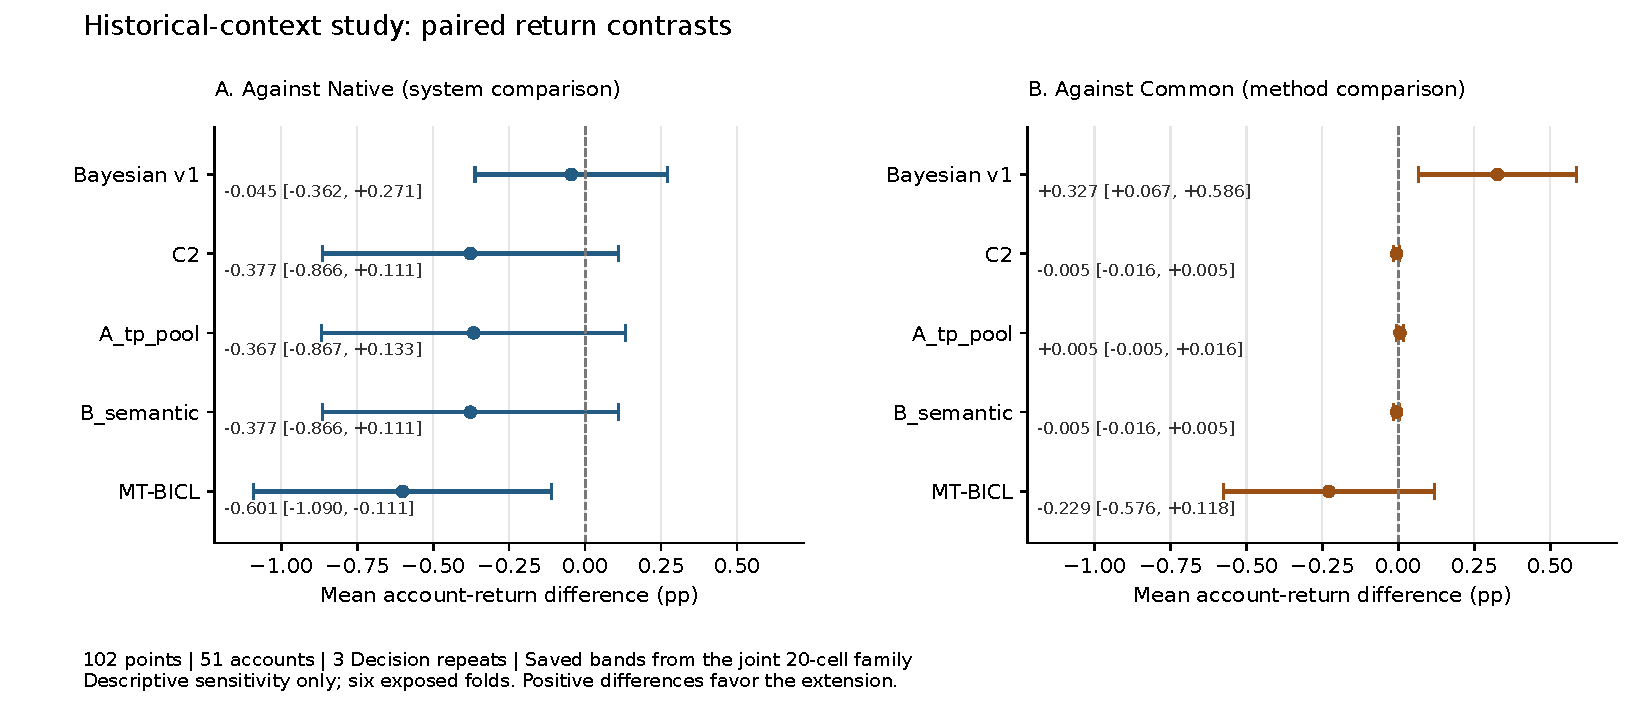
\includegraphics[width=\linewidth,height=0.72\textheight,keepaspectratio]{../assets/figures/F09_return_contrasts.pdf}
\caption{Figure F09. Paired mean account-return contrasts against Native and Common, with saved joint-family descriptive bands.}\label{fig:F09}\end{figure}

\textbf{Figure F09. Paired mean account-return differences.} Both panels use
the same horizontal pp scale. Positive differences favor the extension.
All ten return contrasts are shown; their BA counterparts are retained in
B06d. The plotted estimates and band endpoints are read directly from
the locked result, without new resampling. Editable plotting source,
\href{../assets/figures/F09_return_contrasts.pdf}{vector PDF} and
\href{../assets/figures/F09_return_contrasts.png}{PNG preview} accompany the
\href{../assets/figures/F09_return_contrasts.py}{SVG/source code}.

Bayesian v1 improves on Common by \textbf{+0.327 pp} in mean account return
with band {[}0.067, 0.586{]} pp, and by \textbf{+4.130 pp} in BA with band
{[}2.011, 6.249{]} pp.~Against Native, however, its return difference is
\ensuremath{-}0.045 pp with band {[}\ensuremath{-}0.362, 0.271{]} pp, and BA difference is \ensuremath{-}1.749 pp
with band {[}\ensuremath{-}6.374, 2.876{]} pp.~Thus the favorable Common-based comparison
does not establish an advantage over Native. It also does not establish
profitability: the Bayesian v1 mean return remains negative.

The small C2/A\_\allowbreak{}tp\_\allowbreak{}pool/B\_\allowbreak{}semantic return differences against Common have
bands crossing zero and mostly reflect retained fallback slots. C2 and
B\_\allowbreak{}semantic have adverse BA bands against Native, entirely below zero at
displayed precision. MT-BICL's return difference against Native is
\ensuremath{-}0.601 pp with band {[}\ensuremath{-}1.090, \ensuremath{-}0.111{]} pp; its BA band spans zero.
Against Common, both MT-BICL bands span zero. These unfavorable and
endpoint-dependent results remain visible. A band excluding zero here
is a feature of a saved descriptive sensitivity construction on six
exposed folds, not a calibrated confirmatory test, a causal effect or a
forecast of future trading performance.

\subsection{Descriptive bridge to anchor and MT policy}\label{s:5d343276184e37a8}

\textbf{Table B06e. Native \ensuremath{\rightarrow} Common \ensuremath{\rightarrow} Fact Anchor \ensuremath{\rightarrow} MT-BICL bridge.} Each row
is the method minus the stated predecessor, over 306 paired final-action
slots on the same 102 points. Returns use 51 accounts and three repeats;
BA uses the within-repeat estimator. Agreement is a count of identical
final actions, not independent market observations. No unrecorded bridge
band is added.\footnote{ED07 \texttt{bridge} and ED16 final actions; CL162, ledger §10.9. Only saved bridge differences and agreement counts are shown; no causal student decomposition or fabricated bridge interval.}

\begingroup
\small
\setstretch{1.05}
\setlength{\tabcolsep}{3pt}

\begin{longtable}[]{@{}
  >{\raggedright\arraybackslash}p{(\linewidth - 8\tabcolsep) * \real{0.2000}}
  >{\raggedright\arraybackslash}p{(\linewidth - 8\tabcolsep) * \real{0.2000}}
  >{\raggedright\arraybackslash}p{(\linewidth - 8\tabcolsep) * \real{0.2000}}
  >{\raggedright\arraybackslash}p{(\linewidth - 8\tabcolsep) * \real{0.2000}}
  >{\raggedright\arraybackslash}p{(\linewidth - 8\tabcolsep) * \real{0.2000}}@{}}
\caption{Table B06e. Native \ensuremath{\rightarrow} Common \ensuremath{\rightarrow} Fact Anchor \ensuremath{\rightarrow} MT-BICL bridge.}\label{tab:05_experiments:22}\tabularnewline
\toprule\noalign{}
Predecessor
 & Method
 & Return difference (pp)
 & BA difference (pp)
 & Same final actions
 \\
\midrule\noalign{}
\endfirsthead
\toprule\noalign{}
Predecessor
 & Method
 & Return difference (pp)
 & BA difference (pp)
 & Same final actions
 \\
\midrule\noalign{}
\endhead
\bottomrule\noalign{}
\endlastfoot
Native & Common & -0.372 & -5.879 & 273/306 \\
Common & Fact Anchor & -0.262 & -3.229 & 273/306 \\
Fact Anchor & MT-BICL & 0.033 & 0.433 & 302/306 \\
\end{longtable}

\endgroup

Moving from Native to Common changes both the alpha projection and the
prompt instructions. The return and BA decrease in this bridge, while
273/306 final actions agree. Adding Fact Anchor to Common is associated
with further decreases and the same agreement count, 273/306. These are
combined comparisons involving recorded responses, not isolated numeric
veto effects.

MT-BICL improves on Fact Anchor by only +0.033 pp in return and +0.433 pp
in BA, with \textbf{302/306 identical final actions}. The final-action system
is therefore very close to the anchor on this collection. This observation
does not identify how much is attributable separately to the student,
historical tasks, teacher or utility policy. Section 5.8 examines the
recorded bypasses and proposal--anchor disagreements before interpreting
the MT result.

\section{Mechanisms, case studies and robustness}\label{s:300d164b42208c53}

\subsection{Historical support and recorded context}\label{s:0ac98e073df9fab3}

The coverage analysis separates bank availability, a method's readiness
gate, a new raw response and a change in final action. These stages are
not interchangeable. The frozen same-symbol signal bank covers the 48
CORE4 points; the other 54 points have no same-symbol bank. The latter
reuse Common at the same repeat for all four signal-prior methods.

\textbf{Table B07a. Signal-prior support, counted once per point at repeat 0.}
All three repeats have the same support partition. ``Ready'' is the recorded
conditional request status; v1 does not apply the C2 quality gate. Visible
examples count what the request exposes, not every eligible historical
record. Bank-covered insufficient points and no-bank points are distinct
fallback reasons.\footnote{ED16 prediction fields linked by \texttt{trace\_\allowbreak{}sha256} to ED40; ED07 support summaries; CL163--CL165, ledger §10.10. Descriptor summaries are direct counts/median/range of stored fields, not new forecasts or performance estimates. Missing fields and overlapping gate reasons are preserved.}

\begin{landscape}
\begingroup
\fontsize{9}{11}\selectfont
\setstretch{1.05}
\setlength{\tabcolsep}{3pt}

\begin{longtable}[]{@{}
  >{\raggedright\arraybackslash}p{(\linewidth - 12\tabcolsep) * \real{0.1429}}
  >{\raggedright\arraybackslash}p{(\linewidth - 12\tabcolsep) * \real{0.1429}}
  >{\raggedright\arraybackslash}p{(\linewidth - 12\tabcolsep) * \real{0.1429}}
  >{\raggedright\arraybackslash}p{(\linewidth - 12\tabcolsep) * \real{0.1429}}
  >{\raggedright\arraybackslash}p{(\linewidth - 12\tabcolsep) * \real{0.1429}}
  >{\raggedright\arraybackslash}p{(\linewidth - 12\tabcolsep) * \real{0.1429}}
  >{\raggedright\arraybackslash}p{(\linewidth - 12\tabcolsep) * \real{0.1426}}@{}}
\caption{Table B07a. Signal-prior support, counted once per point at repeat 0.}\label{tab:05_experiments:23}\tabularnewline
\toprule\noalign{}
Signal prior
 & Bank-covered
 & No same-symbol bank
 & Conditional READY
 & Covered insufficient
 & Points with new reply
 & Visible examples
 \\
\midrule\noalign{}
\endfirsthead
\toprule\noalign{}
Signal prior
 & Bank-covered
 & No same-symbol bank
 & Conditional READY
 & Covered insufficient
 & Points with new reply
 & Visible examples
 \\
\midrule\noalign{}
\endhead
\bottomrule\noalign{}
\endlastfoot
Bayesian v1 & 48 & 54 & Not applied & Not applied & 48 & 3 on 48 points \\
C2 & 48 & 54 & 1 & 47 & 1 & 0 on all 48 points \\
A\_\allowbreak{}tp\_\allowbreak{}pool & 48 & 54 & 8 & 40 & 8 & 0 on all 48 points \\
B\_\allowbreak{}semantic & 48 & 54 & 1 & 47 & 1 & 0 on all 48 points \\
\end{longtable}

\endgroup
\end{landscape}

Bayesian v1 retrieves three examples on each of its 48 active points.
Among those points, its recorded retrieval regime is CONSOLIDATION for
40, BULL for four and CHOPPY for four. These are the signal-retrieval
regimes; they must not be relabeled as the separate VN-Index/HMM regimes
used by numerical MT context. The same inputs can have different regime
labels from the two implemented sources, as EX01 demonstrates.

For C2 and B\_\allowbreak{}semantic, only one point is READY; A\_\allowbreak{}tp\_\allowbreak{}pool has eight.
Their READY requests have zero visible examples and expose ready
statistics. Thus a conditional call here does not establish that a
full three-example prompt was used. Among the 48 bank-covered points,
LOW\_\allowbreak{}POPULATION\_\allowbreak{}SUPPORT appears in forty request reason lists for each
conditional method; QUERY\_\allowbreak{}FEATURE\_\allowbreak{}UNAVAILABLE appears in ten. These
reason counts overlap and do not partition the cohort. No-bank coverage
and conditional readiness explain why metrics in Section 5.7 can remain
close to Common without showing that two fully active methods behave
identically.

\textbf{Table B07b. Available context descriptors and probability outputs.}
Age/similarity are summaries of recorded per-point fields, counted once
at repeat 0 and checked unchanged across repeats. Age is the recorded
mean example age in calendar days; similarity follows the signal scorer,
not a calibrated probability. The MT rows describe a different context
representation. NA means that the indicated cohort field is not available
in the U09 prediction export, rather than a numerical zero.\footnote{ED16 prediction fields linked by \texttt{trace\_\allowbreak{}sha256} to ED40; ED07 support summaries; CL163--CL165, ledger §10.10. Descriptor summaries are direct counts/median/range of stored fields, not new forecasts or performance estimates. Missing fields and overlapping gate reasons are preserved.}

\begingroup
\small
\setstretch{1.05}
\setlength{\tabcolsep}{3pt}

\begin{longtable}[]{@{}
  >{\raggedright\arraybackslash}p{(\linewidth - 4\tabcolsep) * \real{0.2400}}
  >{\raggedright\arraybackslash}p{(\linewidth - 4\tabcolsep) * \real{0.3900}}
  >{\raggedright\arraybackslash}p{(\linewidth - 4\tabcolsep) * \real{0.3700}}@{}}
\caption{Table B07b. Available context descriptors and probability outputs.}\label{tab:05_experiments:24}\tabularnewline
\toprule\noalign{}
Recorded quantity
 & Unique-point support
 & Saved-field summary
 \\
\midrule\noalign{}
\endfirsthead
\toprule\noalign{}
Recorded quantity
 & Unique-point support
 & Saved-field summary
 \\
\midrule\noalign{}
\endhead
\bottomrule\noalign{}
\endlastfoot
v1 effective K & 48 & 3 on every active point \\
v1 mean example age (days) & 48 & median 1291.833; range {[}441.667, 2026.000{]} \\
v1 mean similarity & 48 & median 0.833; range {[}0.500, 1.000{]} \\
MT effective K & 102 & 3 on 86 points; 0 on 16 points \\
MT mean age / similarity (U09 export) & 0 & NA / NA \\
MT numeric probability & 86 & 258 slots; supported-only Brier 0.205811 \\
MT teacher probability & 66 & 198 slots; supported-only Brier 0.212024 \\
Prior regret (U09 export) & 0 & NA: NOT\_\allowbreak{}RECORDED\_\allowbreak{}IN\_\allowbreak{}LOCKED\_\allowbreak{}TRACE \\
\end{longtable}

\endgroup

The v1 age range, extending beyond five years for some point-level means,
shows that temporal maturity does not ensure recency or relevance. Its
similarity values belong to the recorded signal-match rule. Neither
those values nor the observed regime labels alone demonstrate a regime
mechanism: matched no-regime/recent/random retrieval results are absent
from this hosted collection. The MT age/similarity cells in this export
are left unavailable; the detailed numerical-context example in Chapter 4
does not supply a cohort summary for those missing export fields. Prior
regret is also not recorded in the locked prediction fields and is not
invented as an explanation of performance.

\subsection{Anchor-relative revisions and probability outputs}\label{s:788636854f37893f}

\begin{figure}[htbp]\centering
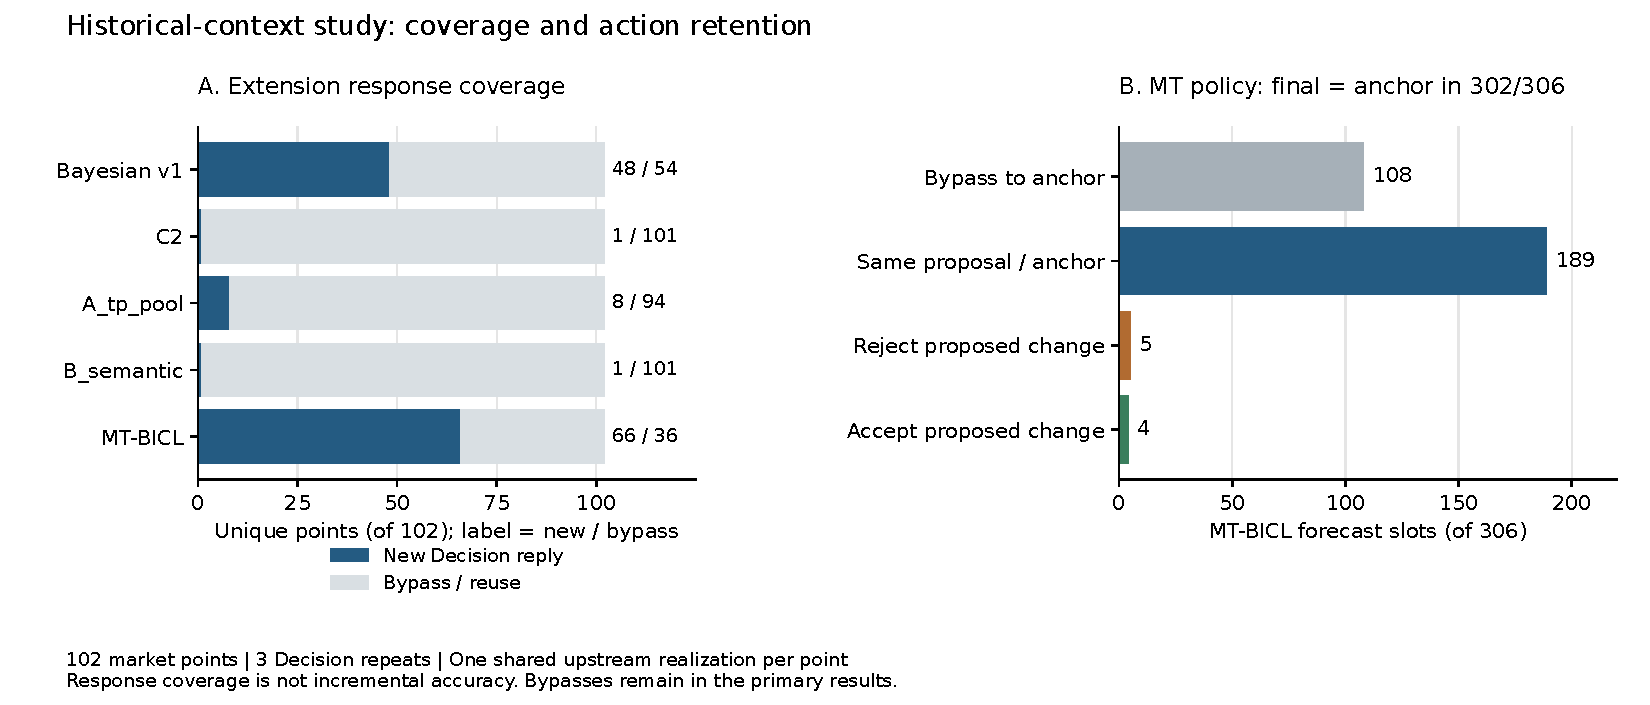
\includegraphics[width=\linewidth,height=0.72\textheight,keepaspectratio]{../assets/figures/F10_coverage_actions.pdf}
\caption{Figure F10. New-response coverage and MT policy counts with their separate denominators.}\label{fig:F10}\end{figure}

\textbf{Figure F10. Response coverage and final-action retention.} The left
panel counts unique points; the right counts 306 MT forecast slots.
All bypasses remain in primary metrics. The chart is drawn from saved
summary counts, with \href{../assets/figures/F10_coverage_actions.pdf}{PDF},
\href{../assets/figures/F10_coverage_actions.png}{PNG} and
\href{../assets/figures/F10_coverage_actions.py}{plotting source}.

\textbf{Table B07c. Complete MT policy path counts.} The five mutually exclusive
reason categories sum to 306 slots. A support bypass has no new revision
response; it is not a rejected malformed response. Counts below are the
actual saved reason counts.\footnote{ED07 \texttt{summary.\allowbreak{}MT\_\allowbreak{}BICL.\allowbreak{}policy\_\allowbreak{}reasons}, \texttt{calibration}, ED16 slot-level actions/flags/quantiles and the Chapter 4 policy contract; CL166--CL168, ledger §10.10. The 302/306 agreement includes bypasses and rejected changes; no causal decomposition or matched-probability comparison is claimed.}

\begingroup
\small
\setstretch{1.05}
\setlength{\tabcolsep}{3pt}

\begin{longtable}[]{@{}
  >{\raggedright\arraybackslash}p{(\linewidth - 4\tabcolsep) * \real{0.2400}}
  >{\raggedright\arraybackslash}p{(\linewidth - 4\tabcolsep) * \real{0.3900}}
  >{\raggedright\arraybackslash}p{(\linewidth - 4\tabcolsep) * \real{0.3700}}@{}}
\caption{Table B07c. Complete MT policy path counts.}\label{tab:05_experiments:25}\tabularnewline
\toprule\noalign{}
Saved reason
 & Forecast slots
 & Final-action relationship
 \\
\midrule\noalign{}
\endfirsthead
\toprule\noalign{}
Saved reason
 & Forecast slots
 & Final-action relationship
 \\
\midrule\noalign{}
\endhead
\bottomrule\noalign{}
\endlastfoot
BYPASS\_\allowbreak{}QUERY\_\allowbreak{}FEATURE\_\allowbreak{}UNAVAILABLE & 48 & Retain anchor; no revision reply \\
BYPASS\_\allowbreak{}UTILITY\_\allowbreak{}UNSUPPORTED & 60 & Retain anchor; no revision reply \\
KEEP\_\allowbreak{}PROPOSED\_\allowbreak{}SAME & 189 & Proposal already equals anchor \\
REJECT\_\allowbreak{}NONPOSITIVE\_\allowbreak{}Q10\_\allowbreak{}DELTA\_\allowbreak{}U & 5 & Reject change; retain anchor \\
ACCEPT\_\allowbreak{}POSITIVE\_\allowbreak{}Q10\_\allowbreak{}DELTA\_\allowbreak{}U & 4 & Change from anchor \\
\end{longtable}

\endgroup

Numerical features are available on 86 points, but only 66 are eligible
for a hosted MT revision: twenty further points lack supported utility.
The sixteen feature-unavailable points and twenty utility-unsupported
points produce 48 and 60 bypass slots, respectively. The recorded
effective K is three on 86 points and zero on sixteen; K alone therefore
does not certify eligibility or a raw revision response.

Fact Anchor records valid fact assertions in all 306 slots and no numeric
veto. Among the 198 eligible MT responses, fact assertions are also valid
in every slot: 189 proposals map to the existing anchor action, and nine
differ. The utility policy rejects five of those nine changes and accepts
four, leaving 302/306 final actions equal to the anchor. The MT export's
false assertion-validity flag on 108 bypass slots is not evidence of
108 malformed responses: those slots have no new revision response.

As defined in Section 4.8.6, a CASH\ensuremath{\rightarrow}LONG change needs Q10(U)\textgreater0, whereas
a LONG\ensuremath{\rightarrow}CASH change needs \ensuremath{-}Q90(U)\textgreater0. U09's \texttt{utility\_\allowbreak{}q10} and \texttt{utility\_\allowbreak{}q90}
are utility-distribution fields, not automatically Q10 of the
anchor-relative change. Consequently, an accepted switch to CASH can
coexist with a negative recorded Q10(U); the upper quantile supplies the
relevant test. The case analysis below checks both action direction and
the policy record rather than inferring a veto from a quantile's sign.

The saved numeric-probability Brier score is 0.205811 on 258 supported
slots representing 86 unique points. The teacher-probability score is
0.212024 on 198 slots representing 66 points. These are different support
sets and numerical outputs; the two scores do not establish that one
predictor outperforms the other on matched support. Repeated points are
not independent calibration samples, and no LLM verbal confidence is
mapped into a probability. Unsupported observations remain in the main
action results, although Brier is defined only on the recorded supported
probabilities.\footnote{ED07 \texttt{summary.\allowbreak{}MT\_\allowbreak{}BICL.\allowbreak{}policy\_\allowbreak{}reasons}, \texttt{calibration}, ED16 slot-level actions/flags/quantiles and the Chapter 4 policy contract; CL166--CL168, ledger §10.10. The 302/306 agreement includes bypasses and rejected changes; no causal decomposition or matched-probability comparison is claimed.}

The observed policy suppresses most deviations from Fact Anchor, but
the collection has no matched hosted No\_\allowbreak{}utility or Plain\_\allowbreak{}revision panel
to estimate the utility gate's isolated performance effect. Similarly,
the near-anchor final actions cannot identify a separate student benefit.
The bridge is descriptive of the implemented combined system.

\subsection{Traceable cases selected by the declared rule}\label{s:87c6a7dca7101b3c}

The case study applies the editorial rule in ledger Section 7.7 after the
study was frozen. It fixes repeat 0 and verifies complete shared,
prepare, forecast and outcome sources before selection. All 102 points
have the required records for all eight research roles. Within each group,
the first point in ascending \texttt{(date, symbol)} order is selected. This is
an explanatory selection rule, not a preregistered performance analysis.

\textbf{Table B07d. Case selection and candidate denominators.} Sufficient
context requires MT eligibility and no v1 bypass. Insufficient support
requires a bypass and explicit INSUFFICIENT\_\allowbreak{}EVIDENCE status in at least
one of C2/A\_\allowbreak{}tp\_\allowbreak{}pool/B\_\allowbreak{}semantic; ties use that stated method order.
Disagreement requires a raw MT proposal mapped to LONG/CASH to differ
from its anchor. A veto requires the recorded utility rejection to change
that mapped raw proposal to the final action. An incorrect case has a
LONG/DOWN or CASH/UP final action in at least one research role; ties use
the role order in B06a. Only the last predicate uses outcomes, deliberately
to illustrate an error.\footnote{Selection rule EX01\_\allowbreak{}SELECTION\_\allowbreak{}V1 and ledger §7.7; ED16/40 plus U08 source chains in §10.11; CL169. All sources were checked before applying the five predicates; no favorable repeat or outcome-based selection outside the declared error group.}

\begingroup
\small
\setstretch{1.05}
\setlength{\tabcolsep}{3pt}

\begin{longtable}[]{@{}
  >{\raggedright\arraybackslash}p{(\linewidth - 6\tabcolsep) * \real{0.1800}}
  >{\raggedright\arraybackslash}p{(\linewidth - 6\tabcolsep) * \real{0.2700}}
  >{\raggedright\arraybackslash}p{(\linewidth - 6\tabcolsep) * \real{0.2800}}
  >{\raggedright\arraybackslash}p{(\linewidth - 6\tabcolsep) * \real{0.2700}}@{}}
\caption{Table B07d. Case selection and candidate denominators.}\label{tab:05_experiments:26}\tabularnewline
\toprule\noalign{}
Declared group
 & Candidate points
 & Selected point
 & Displayed role
 \\
\midrule\noalign{}
\endfirsthead
\toprule\noalign{}
Declared group
 & Candidate points
 & Selected point
 & Displayed role
 \\
\midrule\noalign{}
\endhead
\bottomrule\noalign{}
\endlastfoot
Sufficient context & 29 & FPT-2023-07-03 & MT-BICL \\
Insufficient conditional support & 47 & FPT-2023-07-03 & C2 \\
Proposal / anchor disagreement & 5 & HVN-2024-07-01 & MT-BICL \\
Policy veto of raw proposal & 2 & MWG-2024-09-20 & MT-BICL \\
Incorrect final action & 52 & CMG-2023-07-03 & Native \\
\end{longtable}

\endgroup

The groups overlap: EX01 is the first sufficient-context case and the
first conditional-insufficiency case. The 52-point incorrect-case
denominator counts points where any research role errs at repeat 0; it
is not an error count for one method or for all three repeats. Likewise,
the two veto cases are the repeat-0 subset, distinct from the five rejected
MT changes across all repeats in B07c.

\textbf{Table B07e. Cutoff facts from the recorded numerical audit packets.}
Prices and moving averages use the packet's source unit, thousand VND.
All packets end at the stated cutoff, use 45 bars and record missing
sentiment. For the Native error case, this packet is an associated audit
view; Native did not receive the MT fact-packet interface. The table does
not assert identical prompts across profiles.\footnote{U08 raw member/hash bindings CT01--CT30 in ledger §10.11, linked to ED16 predictions by point/method/repeat, shared output, policy and request IDs; EX01 details also in §7.2--§7.6. CL170--CL173. Prepared packets are inputs/audit views, forecast policies precede the outcome barrier, and outcome returns retain the canonical two-way costs.}

\begin{landscape}
\begingroup
\fontsize{9}{11}\selectfont
\setstretch{1.05}
\setlength{\tabcolsep}{3pt}

\begin{longtable}[]{@{}
  >{\raggedright\arraybackslash}p{(\linewidth - 12\tabcolsep) * \real{0.1429}}
  >{\raggedright\arraybackslash}p{(\linewidth - 12\tabcolsep) * \real{0.1429}}
  >{\raggedright\arraybackslash}p{(\linewidth - 12\tabcolsep) * \real{0.1429}}
  >{\raggedright\arraybackslash}p{(\linewidth - 12\tabcolsep) * \real{0.1429}}
  >{\raggedright\arraybackslash}p{(\linewidth - 12\tabcolsep) * \real{0.1429}}
  >{\raggedright\arraybackslash}p{(\linewidth - 12\tabcolsep) * \real{0.1429}}
  >{\raggedright\arraybackslash}p{(\linewidth - 12\tabcolsep) * \real{0.1426}}@{}}
\caption{Table B07e. Cutoff facts from the recorded numerical audit packets.}\label{tab:05_experiments:27}\tabularnewline
\toprule\noalign{}
Point
 & Close
 & SMA20
 & MACD / Signal
 & MACD / zero
 & Price / SMA20
 & Sentiment
 \\
\midrule\noalign{}
\endfirsthead
\toprule\noalign{}
Point
 & Close
 & SMA20
 & MACD / Signal
 & MACD / zero
 & Price / SMA20
 & Sentiment
 \\
\midrule\noalign{}
\endhead
\bottomrule\noalign{}
\endlastfoot
CMG-2023-07-03 & 29.740 & 29.380 & BELOW & POSITIVE & ABOVE & Unavailable \\
FPT-2023-07-03 & 48.180 & 47.568 & BELOW & POSITIVE & ABOVE & Unavailable \\
HVN-2024-07-01 & 27.190 & 24.952 & BELOW & POSITIVE & ABOVE & Unavailable \\
MWG-2024-09-20 & 65.140 & 65.521 & BELOW & POSITIVE & BELOW & Unavailable \\
\end{longtable}

\endgroup
\end{landscape}

\textbf{Table B07f. Raw proposals, anchors and final actions.} Every row is
repeat 0. SHORT maps to CASH. NA denotes no raw response or no applicable
anchor; a fallback's final LONG is not an invented raw LONG response.
The full policy reason and request identity are retained in the ledger.
Query outcomes were joined only after all twenty-four research forecasts
for the point had completed durably.\footnote{U08 raw member/hash bindings CT01--CT30 in ledger §10.11, linked to ED16 predictions by point/method/repeat, shared output, policy and request IDs; EX01 details also in §7.2--§7.6. CL170--CL173. Prepared packets are inputs/audit views, forecast policies precede the outcome barrier, and outcome returns retain the canonical two-way costs.}

\begingroup
\small
\setstretch{1.05}
\setlength{\tabcolsep}{3pt}

\begin{longtable}[]{@{}
  >{\raggedright\arraybackslash}p{(\linewidth - 10\tabcolsep) * \real{0.1667}}
  >{\raggedright\arraybackslash}p{(\linewidth - 10\tabcolsep) * \real{0.1667}}
  >{\raggedright\arraybackslash}p{(\linewidth - 10\tabcolsep) * \real{0.1667}}
  >{\raggedright\arraybackslash}p{(\linewidth - 10\tabcolsep) * \real{0.1667}}
  >{\raggedright\arraybackslash}p{(\linewidth - 10\tabcolsep) * \real{0.1667}}
  >{\raggedright\arraybackslash}p{(\linewidth - 10\tabcolsep) * \real{0.1665}}@{}}
\caption{Table B07f. Raw proposals, anchors and final actions.}\label{tab:05_experiments:28}\tabularnewline
\toprule\noalign{}
Point
 & Role
 & Raw
 & Anchor
 & Final
 & Recorded policy path
 \\
\midrule\noalign{}
\endfirsthead
\toprule\noalign{}
Point
 & Role
 & Raw
 & Anchor
 & Final
 & Recorded policy path
 \\
\midrule\noalign{}
\endhead
\bottomrule\noalign{}
\endlastfoot
FPT-2023-07-03 & MT-BICL & LONG & LONG & LONG & Keep same \\
FPT-2023-07-03 & C2 & NA & NA & LONG & Reuse Common \\
HVN-2024-07-01 & MT-BICL & LONG & CASH & LONG & Accept change \\
MWG-2024-09-20 & MT-BICL & LONG & CASH & CASH & Veto change \\
CMG-2023-07-03 & Native & SHORT & NA & CASH & Raw decision \\
\end{longtable}

\endgroup

\textbf{Table B07g. Outcomes disclosed after facts and actions.} Entry is
Open(t+1), exit is Close(t+3), both in VND. Gross/net candidate-LONG
returns and labels are the saved canonical outcomes; they are not returns
earned by a CASH action. A final CASH action earns 0\% under this reference
contract. These single-cycle outcomes are not account or portfolio
returns.\footnote{U08 raw member/hash bindings CT01--CT30 in ledger §10.11, linked to ED16 predictions by point/method/repeat, shared output, policy and request IDs; EX01 details also in §7.2--§7.6. CL170--CL173. Prepared packets are inputs/audit views, forecast policies precede the outcome barrier, and outcome returns retain the canonical two-way costs.}

\begin{landscape}
\begingroup
\fontsize{9}{11}\selectfont
\setstretch{1.05}
\setlength{\tabcolsep}{3pt}

\begin{longtable}[]{@{}
  >{\raggedright\arraybackslash}p{(\linewidth - 14\tabcolsep) * \real{0.1250}}
  >{\raggedright\arraybackslash}p{(\linewidth - 14\tabcolsep) * \real{0.1250}}
  >{\raggedright\arraybackslash}p{(\linewidth - 14\tabcolsep) * \real{0.1250}}
  >{\raggedright\arraybackslash}p{(\linewidth - 14\tabcolsep) * \real{0.1250}}
  >{\raggedright\arraybackslash}p{(\linewidth - 14\tabcolsep) * \real{0.1250}}
  >{\raggedright\arraybackslash}p{(\linewidth - 14\tabcolsep) * \real{0.1250}}
  >{\raggedright\arraybackslash}p{(\linewidth - 14\tabcolsep) * \real{0.1250}}
  >{\raggedright\arraybackslash}p{(\linewidth - 14\tabcolsep) * \real{0.1250}}@{}}
\caption{Table B07g. Outcomes disclosed after facts and actions.}\label{tab:05_experiments:29}\tabularnewline
\toprule\noalign{}
Point
 & Entry date
 & Exit date
 & Entry open (VND)
 & Exit close (VND)
 & Gross (\%)
 & Net (\%)
 & Net label
 \\
\midrule\noalign{}
\endfirsthead
\toprule\noalign{}
Point
 & Entry date
 & Exit date
 & Entry open (VND)
 & Exit close (VND)
 & Gross (\%)
 & Net (\%)
 & Net label
 \\
\midrule\noalign{}
\endhead
\bottomrule\noalign{}
\endlastfoot
CMG-2023-07-03 & 2023-07-04 & 2023-07-06 & 29740 & 30000 & 0.874 & 0.171 & UP \\
FPT-2023-07-03 & 2023-07-04 & 2023-07-06 & 48180 & 48390 & 0.436 & -0.265 & DOWN \\
HVN-2024-07-01 & 2024-07-02 & 2024-07-04 & 27190 & 26950 & -0.883 & -1.574 & DOWN \\
MWG-2024-09-20 & 2024-09-23 & 2024-09-25 & 65140 & 65810 & 1.029 & 0.324 & UP \\
\end{longtable}

\endgroup
\end{landscape}

\textbf{EX01, FPT at 3 July 2023.} This is the running example introduced before
its outcome in Chapter 4. Its v1 context contains three examples, while
C2 has only nineteen population observations, below twenty, and one
conditional observation, below five. C2 therefore reuses the same-repeat
Common LONG without a new raw response. MT has K=3 numerical prior tasks
and three target observations, meets eligibility and proposes the same
LONG as Fact Anchor; no change-quantile test is needed. The recorded
MT Q10(U) is negative, but KEEP\_\allowbreak{}PROPOSED\_\allowbreak{}SAME is the applicable branch.
The two regime sources remain CONSOLIDATION for v1 and BULL for numerical
MT. Its positive gross return of 0.436\% becomes \textbf{\ensuremath{-}0.265\% net}, making
the LONG incorrect under the actual economic label. Sufficient context
and valid fact assertions do not guarantee a correct or profitable action.

\textbf{HVN at 1 July 2024: an accepted disagreement that loses.} The packet
places MACD below Signal, MACD above zero and price above SMA20. MT has
supported numerical context even though HVN has no same-symbol signal
bank; the two memory systems have different domains. Its raw LONG differs
from anchor CASH. The recorded Q10 of the CASH\ensuremath{\rightarrow}LONG utility change is
0.0027822661645950566, above zero, so policy accepts LONG. The later
candidate-LONG return is \textbf{\ensuremath{-}1.574\% net}. This case follows the declared
disagreement predicate and illustrates that a positive model-based lower
quantile is not an ex-post profit guarantee. It cannot establish how the
student would perform without the rest of the pipeline.

\textbf{MWG at 20 September 2024: a genuine veto with a missed UP outcome.}
The packet records MACD below Signal and price below SMA20. MT is eligible
and proposes LONG against anchor CASH, but its recorded change Q10 is
\ensuremath{-}0.020861640105904133. Policy rejects the change and retains CASH. The
later candidate-LONG outcome is \textbf{+0.324\% net}, so CASH is a classification
error and a missed positive cycle, while its realized reference return
is zero. The veto did not incur a trading loss in this case, and it did
not improve the realized label decision. This distinction prevents a
mechanically conservative gate from being described as uniformly helpful.

\textbf{CMG at 3 July 2023: the first incorrect-action case.} Native proposes
SHORT, which maps to CASH; the later candidate-LONG label is UP with
\textbf{+0.171\% net}. This is a missed opportunity under the forecast contract,
not a short sale or a negative CASH return. The associated audit packet
has the same three categorical fact relations as EX01, but the symbol,
source reports and Native profile differ. Similar fact categories therefore
do not imply identical prompts, a common hidden cause or an appropriate
counterfactual comparison between these two points.

These cases expose an active context that fails, an explicit support
fallback, an accepted but losing change, a veto that misses a gain and a
baseline error. Their inclusion explains observed paths; it does not
estimate their frequencies, demonstrate policy benefit or replace the
complete-cohort results.

\subsection{Sensitivity to support and dependence assumptions}\label{s:1579bde3c1aaca22}

The sensitivity analyses reuse saved predictions and retain each study's
estimators. They do not add independent market observations or repair
historical exposure. In the context study, circular block lengths 1 and
3 supplement the primary length-2 construction. Each saved sensitivity
family retains all twenty contrasts and 10,000 jointly finite draws.
CORE4 is a fixed 48-point, 24-account subset, not an alternative primary
cohort. Leaving out one fold or stock changes the included support;
the resulting point estimates are diagnostic perturbations, not new
confirmatory estimates.

\textbf{Table B06f. Context return sensitivity for every extension and baseline.}
Units are pp.~L1/L3 are saved bands around the full-cohort point estimates
in B06d. CORE4 cells give their own estimate {[}band{]}. LOFO/LOSO cells give
the minimum and maximum of the six/nine saved leave-one-out point
differences, not confidence intervals. All five extensions and both
baselines are retained.\footnote{ED07 \texttt{sensitivity} arrays use the exact twenty-cell identity order in \texttt{contrasts}; CL174--CL175, ledger §10.12. L1/L3/CORE4 bands and leave-one-out point vectors are read, not regenerated; min/max summarize saved vectors only.}

\begin{landscape}
\begingroup
\fontsize{9}{11}\selectfont
\setstretch{1.05}
\setlength{\tabcolsep}{3pt}

\begin{longtable}[]{@{}
  >{\raggedright\arraybackslash}p{(\linewidth - 12\tabcolsep) * \real{0.1429}}
  >{\raggedright\arraybackslash}p{(\linewidth - 12\tabcolsep) * \real{0.1429}}
  >{\raggedright\arraybackslash}p{(\linewidth - 12\tabcolsep) * \real{0.1429}}
  >{\raggedright\arraybackslash}p{(\linewidth - 12\tabcolsep) * \real{0.1429}}
  >{\raggedright\arraybackslash}p{(\linewidth - 12\tabcolsep) * \real{0.1429}}
  >{\raggedright\arraybackslash}p{(\linewidth - 12\tabcolsep) * \real{0.1429}}
  >{\raggedright\arraybackslash}p{(\linewidth - 12\tabcolsep) * \real{0.1426}}@{}}
\caption{Table B06f. Context return sensitivity for every extension and baseline.}\label{tab:05_experiments:30}\tabularnewline
\toprule\noalign{}
Baseline
 & Extension
 & L1 band
 & L3 band
 & CORE4 estimate {[}band{]}
 & LOFO point range
 & LOSO point range
 \\
\midrule\noalign{}
\endfirsthead
\toprule\noalign{}
Baseline
 & Extension
 & L1 band
 & L3 band
 & CORE4 estimate {[}band{]}
 & LOFO point range
 & LOSO point range
 \\
\midrule\noalign{}
\endhead
\bottomrule\noalign{}
\endlastfoot
Native & Bayesian v1 & {[}-0.476, 0.385{]} & {[}-0.314, 0.223{]} & 0.350 {[}-0.024, 0.725{]} & {[}-0.145, 0.107{]} & {[}-0.162, 0.133{]} \\
Native & C2 & {[}-0.865, 0.110{]} & {[}-0.720, -0.035{]} & -0.355 {[}-0.843, 0.132{]} & {[}-0.453, -0.206{]} & {[}-0.447, -0.243{]} \\
Native & A\_\allowbreak{}tp\_\allowbreak{}pool & {[}-0.861, 0.127{]} & {[}-0.722, -0.011{]} & -0.333 {[}-0.852, 0.186{]} & {[}-0.441, -0.193{]} & {[}-0.435, -0.231{]} \\
Native & B\_\allowbreak{}semantic & {[}-0.865, 0.110{]} & {[}-0.720, -0.035{]} & -0.355 {[}-0.843, 0.132{]} & {[}-0.453, -0.206{]} & {[}-0.447, -0.243{]} \\
Native & MT-BICL & {[}-1.077, -0.124{]} & {[}-0.949, -0.252{]} & -0.459 {[}-0.975, 0.057{]} & {[}-0.725, -0.471{]} & {[}-0.675, -0.432{]} \\
Common & Bayesian v1 & {[}-0.019, 0.672{]} & {[}0.144, 0.509{]} & 0.694 {[}0.132, 1.257{]} & {[}0.218, 0.397{]} & {[}0.197, 0.370{]} \\
Common & C2 & {[}-0.018, 0.007{]} & {[}-0.013, 0.002{]} & -0.011 {[}-0.034, 0.011{]} & {[}-0.006, 0.000{]} & {[}-0.006, 0.000{]} \\
Common & A\_\allowbreak{}tp\_\allowbreak{}pool & {[}-0.007, 0.018{]} & {[}-0.002, 0.013{]} & 0.011 {[}-0.011, 0.034{]} & {[}0.000, 0.006{]} & {[}0.000, 0.006{]} \\
Common & B\_\allowbreak{}semantic & {[}-0.018, 0.007{]} & {[}-0.013, 0.002{]} & -0.011 {[}-0.034, 0.011{]} & {[}-0.006, 0.000{]} & {[}-0.006, 0.000{]} \\
Common & MT-BICL & {[}-0.578, 0.120{]} & {[}-0.469, 0.012{]} & -0.115 {[}-0.205, -0.026{]} & {[}-0.312, -0.130{]} & {[}-0.260, -0.192{]} \\
\end{longtable}

\endgroup
\end{landscape}

\textbf{Table B06g. Corresponding BA sensitivity, in pp.} The same family
identities, support and display conventions apply. Undefined grouped BA
is never filled with zero or used to remove a primary observation.

\begin{landscape}
\begingroup
\fontsize{9}{11}\selectfont
\setstretch{1.05}
\setlength{\tabcolsep}{3pt}

\begin{longtable}[]{@{}
  >{\raggedright\arraybackslash}p{(\linewidth - 12\tabcolsep) * \real{0.1429}}
  >{\raggedright\arraybackslash}p{(\linewidth - 12\tabcolsep) * \real{0.1429}}
  >{\raggedright\arraybackslash}p{(\linewidth - 12\tabcolsep) * \real{0.1429}}
  >{\raggedright\arraybackslash}p{(\linewidth - 12\tabcolsep) * \real{0.1429}}
  >{\raggedright\arraybackslash}p{(\linewidth - 12\tabcolsep) * \real{0.1429}}
  >{\raggedright\arraybackslash}p{(\linewidth - 12\tabcolsep) * \real{0.1429}}
  >{\raggedright\arraybackslash}p{(\linewidth - 12\tabcolsep) * \real{0.1426}}@{}}
\caption{Table B06g. Corresponding BA sensitivity, in pp.}\label{tab:05_experiments:31}\tabularnewline
\toprule\noalign{}
Baseline
 & Extension
 & L1 band
 & L3 band
 & CORE4 estimate {[}band{]}
 & LOFO point range
 & LOSO point range
 \\
\midrule\noalign{}
\endfirsthead
\toprule\noalign{}
Baseline
 & Extension
 & L1 band
 & L3 band
 & CORE4 estimate {[}band{]}
 & LOFO point range
 & LOSO point range
 \\
\midrule\noalign{}
\endhead
\bottomrule\noalign{}
\endlastfoot
Native & Bayesian v1 & {[}-7.081, 3.584{]} & {[}-5.258, 1.760{]} & -0.351 {[}-10.475, 9.773{]} & {[}-2.694, 0.284{]} & {[}-3.231, -0.414{]} \\
Native & C2 & {[}-11.682, -0.508{]} & {[}-10.054, -2.137{]} & -9.474 {[}-20.432, 1.484{]} & {[}-7.344, -4.119{]} & {[}-7.152, -4.683{]} \\
Native & A\_\allowbreak{}tp\_\allowbreak{}pool & {[}-11.434, 0.110{]} & {[}-10.200, -1.125{]} & -8.596 {[}-20.969, 3.776{]} & {[}-6.798, -3.598{]} & {[}-6.718, -4.186{]} \\
Native & B\_\allowbreak{}semantic & {[}-11.682, -0.508{]} & {[}-10.054, -2.137{]} & -9.474 {[}-20.432, 1.484{]} & {[}-7.344, -4.119{]} & {[}-7.152, -4.683{]} \\
Native & MT-BICL & {[}-20.362, 3.012{]} & {[}-17.868, 0.518{]} & -15.000 {[}-28.388, -1.612{]} & {[}-12.483, -4.820{]} & {[}-9.897, -6.453{]} \\
Common & Bayesian v1 & {[}0.323, 7.937{]} & {[}2.092, 6.168{]} & 8.684 {[}4.472, 12.896{]} & {[}2.910, 5.038{]} & {[}2.277, 5.280{]} \\
Common & C2 & {[}-0.781, 0.348{]} & {[}-0.528, 0.095{]} & -0.439 {[}-1.361, 0.484{]} & {[}-0.273, 0.000{]} & {[}-0.249, 0.000{]} \\
Common & A\_\allowbreak{}tp\_\allowbreak{}pool & {[}-0.348, 0.781{]} & {[}-0.095, 0.528{]} & 0.439 {[}-0.484, 1.361{]} & {[}0.000, 0.273{]} & {[}0.000, 0.249{]} \\
Common & B\_\allowbreak{}semantic & {[}-0.781, 0.348{]} & {[}-0.528, 0.095{]} & -0.439 {[}-1.361, 0.484{]} & {[}-0.273, 0.000{]} & {[}-0.249, 0.000{]} \\
Common & MT-BICL & {[}-12.059, 6.466{]} & {[}-9.588, 3.995{]} & -5.965 {[}-9.604, -2.326{]} & {[}-5.601, 0.572{]} & {[}-4.186, -0.759{]} \\
\end{longtable}

\endgroup
\end{landscape}

Bayesian v1's return difference against Common stays positive under every
saved leave-one-fold-out perturbation, from +0.218 to +0.397 pp, and every
leave-one-stock-out perturbation, from +0.197 to +0.370 pp.~Its L1 band,
however, is \textbf{{[}\ensuremath{-}0.019, 0.672{]} pp}, crossing zero, whereas the primary L2
band is {[}0.067, 0.586{]} pp and L3 gives {[}0.144, 0.509{]} pp.~Thus even the
zero-exclusion description depends on the dependence construction; the
narrower L3 display is not a reason to select it as the principal result.
Against Native, the v1 leave-one-out return differences change sign.

On CORE4, v1 minus Common is +0.694 pp {[}0.132, 1.257{]}, while v1 minus
Native is +0.350 pp {[}\ensuremath{-}0.024, 0.725{]}. This subset contains the signal-bank
domain and changes the comparator population. MT-BICL remains below both
baselines in all saved full-cohort leave-one-out return differences. Its
CORE4 comparison against Common has a negative band, despite the
full-cohort primary band crossing zero. These variations reinforce the
need to specify baseline and population, rather than claiming a general
regime-aware or MT improvement.

\textbf{Table B05h. Component support sensitivities.} These overlapping cohorts
retain the recorded Full/Base predictions and the component account
estimator. They do not share response collections with the context study.
BA is a percentage, return is a percentage and financial means use the
stated number of accounts.\footnote{ED33--ED35 cohort exports; ED28 leave-one-block results; ED41 circular-block rows, ED42 panel-HAC, ED45 strata and ED47 definitions; CL176--CL177, ledger §10.12. Cohorts and stratifications are overlapping, descriptive and retain their recorded endpoints.}

\begin{landscape}
\begingroup
\fontsize{9}{11}\selectfont
\setstretch{1.05}
\setlength{\tabcolsep}{3pt}

\begin{longtable}[]{@{}
  >{\raggedright\arraybackslash}p{(\linewidth - 12\tabcolsep) * \real{0.1429}}
  >{\raggedright\arraybackslash}p{(\linewidth - 12\tabcolsep) * \real{0.1429}}
  >{\raggedright\arraybackslash}p{(\linewidth - 12\tabcolsep) * \real{0.1429}}
  >{\raggedright\arraybackslash}p{(\linewidth - 12\tabcolsep) * \real{0.1429}}
  >{\raggedright\arraybackslash}p{(\linewidth - 12\tabcolsep) * \real{0.1429}}
  >{\raggedright\arraybackslash}p{(\linewidth - 12\tabcolsep) * \real{0.1429}}
  >{\raggedright\arraybackslash}p{(\linewidth - 12\tabcolsep) * \real{0.1426}}@{}}
\caption{Table B05h. Component support sensitivities.}\label{tab:05_experiments:32}\tabularnewline
\toprule\noalign{}
Component cohort
 & Points
 & Accounts
 & Full BA (\%)
 & Base BA (\%)
 & Full return (\%)
 & Base return (\%)
 \\
\midrule\noalign{}
\endfirsthead
\toprule\noalign{}
Component cohort
 & Points
 & Accounts
 & Full BA (\%)
 & Base BA (\%)
 & Full return (\%)
 & Base return (\%)
 \\
\midrule\noalign{}
\endhead
\bottomrule\noalign{}
\endlastfoot
all\_\allowbreak{}102 & 102 & 51 & 52.961 & 49.714 & -0.797 & -0.750 \\
common\_\allowbreak{}eight\_\allowbreak{}96 & 96 & 48 & 50.694 & 48.611 & -0.853 & -0.701 \\
recent\_\allowbreak{}nine\_\allowbreak{}54 & 54 & 27 & 53.077 & 46.667 & -0.728 & -0.953 \\
\end{longtable}

\endgroup
\end{landscape}

Removing BHN gives a 96-point common-eight cohort, with Full's mean return
below Base; restricting to the recent three blocks gives 54 points and
reverses that financial ordering. All six saved component leave-one-block
Full-minus-Base BA differences remain positive, ranging from +0.820 to
+4.918 pp, but their small supports do not establish a stable financial
gain. The stored component circular-block BA intervals for Full minus
Base at lengths 1, 2 and 3 all cross zero. The six panel-HAC accuracy
intervals for the common-eight/recent-nine cohorts at lags 0--2 also all
cross zero. These are different diagnostic constructions and endpoints;
their small-sample reference assumptions are not newly validated here.

\textbf{Table B05i. Recorded component descriptive strata on all 102 points.}
Trend uses Close/SMA60 with \ensuremath{\pm}2\% thresholds. Volatility and liquidity-proxy
groups use trailing 20-session quantities compared with each stock/fold's
train-only median. The latter two stratifications were added after
inference. Rows within a dimension partition the sample; dimensions
overlap. These labels are distinct from the numerical HMM regimes.

\begingroup
\small
\setstretch{1.05}
\setlength{\tabcolsep}{3pt}

\begin{longtable}[]{@{}
  >{\raggedright\arraybackslash}p{(\linewidth - 6\tabcolsep) * \real{0.1800}}
  >{\raggedright\arraybackslash}p{(\linewidth - 6\tabcolsep) * \real{0.2700}}
  >{\raggedright\arraybackslash}p{(\linewidth - 6\tabcolsep) * \real{0.2800}}
  >{\raggedright\arraybackslash}p{(\linewidth - 6\tabcolsep) * \real{0.2700}}@{}}
\caption{Table B05i. Recorded component descriptive strata on all 102 points.}\label{tab:05_experiments:33}\tabularnewline
\toprule\noalign{}
Descriptive stratum
 & Points
 & Full BA (\%)
 & Base BA (\%)
 \\
\midrule\noalign{}
\endfirsthead
\toprule\noalign{}
Descriptive stratum
 & Points
 & Full BA (\%)
 & Base BA (\%)
 \\
\midrule\noalign{}
\endhead
\bottomrule\noalign{}
\endlastfoot
trend: bear & 35 & 43.333 & 41.667 \\
trend: bull & 33 & 47.917 & 53.472 \\
trend: sideways & 34 & 59.486 & 46.245 \\
volatility: high & 33 & 46.538 & 50.385 \\
volatility: low & 69 & 57.018 & 48.465 \\
liquidity\_\allowbreak{}proxy: high & 80 & 49.167 & 48.333 \\
liquidity\_\allowbreak{}proxy: low & 22 & 67.059 & 55.294 \\
\end{longtable}

\endgroup

Full is below Base in the bull and high-volatility strata, while it is
above Base in the sideways and low-volatility strata. This heterogeneity
does not demonstrate an optimized regime-switching strategy: no strategy
was rerun by selecting the favorable strata. Liquidity uses vendor
Close\ensuremath{\times}Volume units and is a proxy rather than authenticated tradable
capacity. Its target-session exposure summaries also exclude the cash
gaps present in full-ledger exposure, so those quantities are not silently
substituted into B05b.

\subsection{Recorded economic execution scenarios}\label{s:50af410a302d2e74}

\textbf{Table B05j. Component Full/Base outcomes in all twelve saved scenarios.}
Each branch/scenario has 51 separate accounts on the original 102-point
schedule. Predictions, original net labels and the fixed three-session
horizon remain unchanged; only execution/account assumptions vary. Return
is mean account return (\%). Blocked values count attempts, not necessarily
unique missed market points. Pending and residual columns count accounts
at the terminal window.\footnote{ED26 policy and ED43/ED44 execution summary/report; CL178, ledger §10.12. All twelve scenario IDs are retained; support, blocked attempts and pending/residual states are copied from saved rows, without relabeling or ledger replay.}

\begingroup
\small
\setstretch{1.05}
\setlength{\tabcolsep}{3pt}

\begin{longtable}[]{@{}
  >{\raggedright\arraybackslash}p{(\linewidth - 10\tabcolsep) * \real{0.1667}}
  >{\raggedright\arraybackslash}p{(\linewidth - 10\tabcolsep) * \real{0.1667}}
  >{\raggedright\arraybackslash}p{(\linewidth - 10\tabcolsep) * \real{0.1667}}
  >{\raggedright\arraybackslash}p{(\linewidth - 10\tabcolsep) * \real{0.1667}}
  >{\raggedright\arraybackslash}p{(\linewidth - 10\tabcolsep) * \real{0.1667}}
  >{\raggedright\arraybackslash}p{(\linewidth - 10\tabcolsep) * \real{0.1665}}@{}}
\caption{Table B05j. Component Full/Base outcomes in all twelve saved scenarios.}\label{tab:05_experiments:34}\tabularnewline
\toprule\noalign{}
Scenario
 & Full return (\%)
 & Base return (\%)
 & Blocked Full/Base
 & Pending Full/Base
 & Residual stock Full/Base
 \\
\midrule\noalign{}
\endfirsthead
\toprule\noalign{}
Scenario
 & Full return (\%)
 & Base return (\%)
 & Blocked Full/Base
 & Pending Full/Base
 & Residual stock Full/Base
 \\
\midrule\noalign{}
\endhead
\bottomrule\noalign{}
\endlastfoot
reference & -0.797 & -0.750 & 0/0 & 0/0 & 0/0 \\
pending\_\allowbreak{}t2 & -0.797 & -0.750 & 0/0 & 0/0 & 0/0 \\
advance\_\allowbreak{}on\_\allowbreak{}demand & -0.797 & -0.750 & 0/0 & 0/0 & 0/0 \\
advance\_\allowbreak{}auto & -0.840 & -0.803 & 0/0 & 0/0 & 0/0 \\
lower\_\allowbreak{}cost & -0.612 & -0.526 & 0/0 & 0/0 & 0/0 \\
higher\_\allowbreak{}cost & -1.211 & -1.249 & 0/0 & 0/0 & 0/0 \\
sell\_\allowbreak{}charge\_\allowbreak{}10bp & -0.843 & -0.805 & 0/0 & 0/0 & 0/0 \\
no\_\allowbreak{}fill\_\allowbreak{}proxy & -0.803 & -0.659 & 1/3 & 0/0 & 0/0 \\
delayed\_\allowbreak{}proxy & -0.766 & -0.621 & 2/4 & 0/1 & 0/0 \\
lot100\_\allowbreak{}cap1pct & -0.745 & -0.602 & 1/3 & 0/0 & 0/0 \\
combined & -1.166 & -1.074 & 3/9 & 0/0 & 0/0 \\
all\_\allowbreak{}entries\_\allowbreak{}missed & 0.000 & 0.000 & 24/29 & 0/0 & 0/0 \\
\end{longtable}

\endgroup

Pending settlement and on-demand advance match the reference returns
in this recorded schedule; that equality is not a general claim that
settlement constraints never matter. Automatic advance adds a hypothetical
financing charge. The lower-cost scenario uses 0.10\% brokerage and 0.05\%
slippage per leg; the higher-cost scenario uses 0.50\% and 0.30\%, respectively.
The reference remains 0.25\% and 0.10\% per leg. The higher-cost scenario
reverses the Full/Base return ordering, illustrating the interaction
between selected actions, exposure and costs.

No-fill and delayed-fill scenarios use zero-volume or single-price daily
bars as ex-post feasibility proxies. The lot/cap scenario assumes lots
of 100 and a 1\% cap on lagged trailing-20-session mean vendor Volume.
These are hypothetical planning constraints, not authenticated partial
fills or evidence that a strategy knew queue conditions at the open.
Financing assumes 15\% annually on an ACT/365 basis; it is a stress input,
not a current broker quote. The same account window includes at most five
observed tail sessions; missing maturity dates are not manufactured.

For Base, the delayed proxy leaves one account with pending cash. Full
and Base have no residual stock accounts in these displayed scenarios;
other variants retain their own saved terminal states. The all-entries-
missed control returns zero by avoiding all purchases, not by predicting
successfully. A no-fill screen can avoid losses or miss gains, so its
scenario envelope is not a mathematical worst-case bound. The execution
report retains \textbf{zero execution-certified fills}. This component
sensitivity does not validate venue rules for every historical date or
supply a corresponding execution study for the hosted context methods.

\subsection{Recorded resource use and unavailable costs}\label{s:d6e23446b902a0bb}

\textbf{Table B07h. Resource ledgers with their original scopes.} The component
source ledger includes inherited requests beyond the selected minimal
responses, so it must not be added to the new-request row as the measured
cost of exactly 375 Decision executions. Tokens are SDK-observed usage;
missing error usage is not imputed as zero billed usage. Latency sums are
recorded request durations, not experiment wall-clock time or a matched
method-level speed comparison.\footnote{ED18 component costs, ED07 telemetry and ED46 U08 wire index with its hashed HTTP members; CL179--CL180, ledger §10.12. Duration summaries use finite saved timestamps, exclude carry, preserve two untimed UNKNOWN attempts and provide no billing or deployment certification.}

\begingroup
\small
\setstretch{1.05}
\setlength{\tabcolsep}{3pt}

\begin{longtable}[]{@{}
  >{\raggedright\arraybackslash}p{(\linewidth - 10\tabcolsep) * \real{0.1667}}
  >{\raggedright\arraybackslash}p{(\linewidth - 10\tabcolsep) * \real{0.1667}}
  >{\raggedright\arraybackslash}p{(\linewidth - 10\tabcolsep) * \real{0.1667}}
  >{\raggedright\arraybackslash}p{(\linewidth - 10\tabcolsep) * \real{0.1667}}
  >{\raggedright\arraybackslash}p{(\linewidth - 10\tabcolsep) * \real{0.1667}}
  >{\raggedright\arraybackslash}p{(\linewidth - 10\tabcolsep) * \real{0.1665}}@{}}
\caption{Table B07h. Resource ledgers with their original scopes.}\label{tab:05_experiments:35}\tabularnewline
\toprule\noalign{}
Ledger scope
 & Attempts
 & Success / HTTP 200
 & Errors / other status
 & Observed prompt / completion tokens
 & Duration sum (s)
 \\
\midrule\noalign{}
\endfirsthead
\toprule\noalign{}
Ledger scope
 & Attempts
 & Success / HTTP 200
 & Errors / other status
 & Observed prompt / completion tokens
 & Duration sum (s)
 \\
\midrule\noalign{}
\endhead
\bottomrule\noalign{}
\endlastfoot
Component new requests & 194 & 182 & 12 & 293,885 / 158,161 & 375.304 \\
Component inherited source ledger & 455 & 433 & 22 & 769,443 / 182,575 & 987.375 \\
Context research HTTP & 1702 & 1505 & 197 non-200 / UNKNOWN & 2,986,930 total observed & 4056.744 \\
\end{longtable}

\endgroup

The context ledger has 1,702 HTTP attempts: 1,505 status-200, 194 status-429,
one status-503 and two UNKNOWN records. HTTP successes are not the same
denominator as the 1,290 retained raw Decision responses. The observed
token total is 2,986,930; the 9,177 tokens reserved for UNKNOWN attempts
are accounting headroom, not observed generation. The 503 carried
historical ledger entries are excluded from these research-attempt
counts and timings.

Of the 1,702 context attempts, 1,700 have both recorded start and completion
timestamps. Their elapsed-duration sum is 4,056.744 seconds, median
1.715 seconds and range {[}0.554, 31.819{]} seconds; the two UNKNOWN attempts
have no complete duration. These direct timestamp summaries include the
recorded HTTP scopes and do not measure end-to-end scheduling, cooldowns,
offline training, data acquisition or an isolated method's latency.

Monetary API bills, verified per-role billed usage and a matched end-to-end
latency comparison are unavailable. No currency cost is inferred from
current pricing or token reservations. The saved analysis itself records
zero new API calls; reading and formatting these artifacts also adds no
inference. Resource reuse and checkpointability are engineering properties,
while financial usefulness remains subject to the negative returns and
scope limits already reported.

\section{Unperformed ablations and threats to validity}\label{s:7abb5e08a08c44da}

\subsection{Interventions without a completed matched result}\label{s:51f776e45704e55e}

The implementation contains more builders and research options than the
eight hosted roles evaluated here. The completed component panel and the
Common--Anchor--MT bridge do not fill those experimental gaps. Table B06h
records what remains unmeasured so that method descriptions in Chapter 4
are not read as evidence of isolated performance gains.\footnote{ED07 \texttt{deferred\_\allowbreak{}panels}, completed intervention scopes ED05/37 and Chapter 4 method contracts; CL181, ledger §10.13. Implemented builders, offline tests and separate component panels are distinguished from matched hosted performance observations.}

\textbf{Table B06h. Missing matched interventions.} ``Unperformed'' refers to a
matched hosted comparison in the locked historical-context collection,
not a claim that no related code, offline check or separate component
experiment exists. These are remaining research questions, not experiments
conducted during thesis writing.

\begingroup
\small
\setstretch{1.05}
\setlength{\tabcolsep}{3pt}

\begin{longtable}[]{@{}
  >{\raggedright\arraybackslash}p{(\linewidth - 4\tabcolsep) * \real{0.2400}}
  >{\raggedright\arraybackslash}p{(\linewidth - 4\tabcolsep) * \real{0.3900}}
  >{\raggedright\arraybackslash}p{(\linewidth - 4\tabcolsep) * \real{0.3700}}@{}}
\caption{Table B06h. Missing matched interventions.}\label{tab:05_experiments:36}\tabularnewline
\toprule\noalign{}
Intervention
 & Recorded status / related evidence
 & Effect not identified
 \\
\midrule\noalign{}
\endfirsthead
\toprule\noalign{}
Intervention
 & Recorded status / related evidence
 & Effect not identified
 \\
\midrule\noalign{}
\endhead
\bottomrule\noalign{}
\endlastfoot
Random / recent / similarity / Bayesian retrieval, matched bank and budget & DEFERRED; zero matched hosted retrieval-ablation slots & Retrieval ranking and regime conditioning alone \\
Signal-prior statistics only / examples only / no regime & DEFERRED; conditional methods have different readiness masks & Incremental value of examples, statistics or regime labels \\
Plain\_\allowbreak{}revision / no numerical prior & No matched hosted role; builders do not supply a response comparison & Added numerical historical context under the same revision interface \\
No\_\allowbreak{}utility / Utility\_\allowbreak{}only & DEFERRED matched panel; combined MT policy and bridge observed & Isolated utility-policy performance effect \\
No\_\allowbreak{}target / Stats\_\allowbreak{}only and student--teacher separation & DEFERRED matched MT panel; offline model evidence is separate & Target-task and student/teacher contributions to final trading actions \\
Full-scale alpha / sentiment / placebo with matched prompt format & Separate nine-unit factorial and numerical panels only & 102-point isolated component effects without representation confounding \\
Alternative horizons / prospective execution study & No L=5/10 or prospective live-fill result in this collection & Horizon optimization, live profitability or deployment acceptance \\
\end{longtable}

\endgroup

In particular, the four signal-prior branches differ in readiness,
representation and content. Their aggregate comparisons do not isolate
retrieval ranking or regime information while holding all other inputs
fixed. Similarly, only four MT final slots differ from the anchor, but
the study does not observe the alternate hosted outcomes required to
attribute this pattern to the student, target context or utility gate
separately. The numerical factor rules and small factorial panel answer
their own narrower questions.

\subsection{Limits on causal, statistical and external validity}\label{s:884531ae3b8f0e7c}

\hyperref[s:8356fa5ade54dd36]{Appendix E} provides the audit matrix, retained Native counterexamples and source-scoped receipt outcomes, including the unresolved application gate.

\textbf{Temporal causality and provenance.} The recorded native row-wise
causality gate is \textbf{FAIL}, and the whole-system status remains
\textbf{NOT\_\allowbreak{}CERTIFIED\_\allowbreak{}HISTORICAL\_\allowbreak{}EXPLORATORY}. Cutting the input dataframe at
the query date does not ensure that every earlier feature row was
constructed using only its own past. The Common projection addresses a
specific alpha path; it does not certify all inherited inputs, news,
memory features or Native behavior. The frozen result must retain this
limitation rather than silently replacing its inputs with a repaired
implementation.\footnote{ED15 \texttt{native\_\allowbreak{}rowwise\_\allowbreak{}causal\_\allowbreak{}gate}, \texttt{whole\_\allowbreak{}system\_\allowbreak{}causal\_\allowbreak{}gate}, \texttt{quality\_\allowbreak{}limits}, \texttt{provider\_\allowbreak{}support.\allowbreak{}bank\_\allowbreak{}audit}; ED04 exposure timing; ED08 historical acceptance; ED07 limitations and snapshot cold receipt in ledger §3.4; CL182--CL186, ledger §10.13. Prior receipts are cited within their scope, not described as suites rerun during writing.}

The signal bank and query prices have different recorded provenance.
The audit reports numerical return differences above its threshold in
\textbf{828 of 852 bank records}, with maximum absolute difference
0.04298848884252138 pp.~This is a return-value comparison, \textbf{not a count
of 828 changed labels}. It does not establish that 828 forecast outcomes
are wrong, and it does not justify retroactively relabeling the bank.
The source manifest also records that the original raw signal journals
are unavailable. Membership hashes prove which stored records were used;
they do not independently authenticate how the original bank signals
were generated. Transfer between these sources therefore remains an
explicit limitation.

The study reconstructs historical prices and news from stored vendor and
cache material, rather than independently authenticated contemporaneous
captures at every cutoff. An admissibility check on recorded dates is distinct from independent
authentication that the same content and adjusted series were available
at each historical decision. News content PIT is not certified, and
79/102 points have unavailable sentiment under the recorded study flag.
Missing sentiment is retained rather than treated as observed neutral
news. Numerical fact assertions can be checked against a packet, but
neither that check nor a chart's presence supplies independent financial
ground truth for an agent's explanation.

\textbf{Historical exposure and model uncertainty.} The six folds had already
been examined during development. Analysis and case-selection rules
disclosed after inference do not create an untouched holdout. The
component queue freeze also occurred between its first and last requests;
that timestamp cannot establish a fully prospective evaluation. The
hosted model aliases do not supply an immutable served-weight revision,
and the foundation model's training overlap with these historical periods
is not established. Frozen local student/HMM weights and source hashes
support offline traceability, but do not prove absence of foundation-model
contamination or guarantee byte-identical future hosted replies.

\textbf{Dependence, prompts and estimands.} Nine stocks and three Decision
repeats do not multiply the six exposed temporal clusters into a large
independent sample. Pairing removes avoidable differences in upstream
inputs; it does not supply independent upstream realizations in the
context study or eliminate cross-stock dependence. Descriptive bands
depend on the saved resampling rules, as the L1/L2 difference illustrates.
The small factorial panel has substantial undefined bootstrap support,
and the numerical sign diagnostics rely on unverified symmetry and
exchangeability. These constructions do not establish calibrated coverage,
statistical power or a generalizable causal effect.

Full/Base and Native/Common alter representation and instructions along
with information. Component request order also includes forty paired
order mismatches and nine groups spanning execution epochs; the records
do not establish perfect counterbalancing. Comparisons across studies
add different response collections, estimators, risk definitions and
support. Consequently, neither a classification gain nor lower exposure
can be translated into an isolated information effect, a stronger risk
ratio or a profitable strategy by changing the reporting convention.

\textbf{Sampling and market execution.} The nine-stock sample is purposive;
complete point-in-time index membership and market representativeness
are unresolved. BHN has the shorter eligible history already disclosed.
Corporate actions, dividend treatment, adjusted prices and vendor volume
units have not been independently authenticated for all venue/date
combinations. Daily bars do not reproduce auctions, order-book queues,
partial fills, market impact or actual borrowing/settlement services.
The twelve scenarios are useful stress assumptions with fixed predictions,
but zero execution-certified fills remain zero. Separate 50-million-VND
accounts are not a validated shared-capital portfolio, and SHORT means
CASH throughout. No conclusion extends to actual short selling,
high-frequency execution or a different holding horizon.

\textbf{Acceptance and reproducibility scope.} The historical U08 acceptance
records 718 verified source pins, an observed maximum Decision request
length of 4,750 characters including repair, and at most three HTTP
attempts per execution for that profile. It also explicitly records that
the suite was not rerun at that acceptance step. These observations
support the specific recorded protocol and its prompt/retry accounting;
they do not certify all future profiles or turn a guard into evidence
that every external dependency was causal. The U09 cold-replay receipt
supports offline artifact reproduction with zero new inference. It is
not fresh hosted inference, prospective trading or proof of live
execution quality.\footnote{ED15 \texttt{native\_\allowbreak{}rowwise\_\allowbreak{}causal\_\allowbreak{}gate}, \texttt{whole\_\allowbreak{}system\_\allowbreak{}causal\_\allowbreak{}gate}, \texttt{quality\_\allowbreak{}limits}, \texttt{provider\_\allowbreak{}support.\allowbreak{}bank\_\allowbreak{}audit}; ED04 exposure timing; ED08 historical acceptance; ED07 limitations and snapshot cold receipt in ledger §3.4; CL182--CL186, ledger §10.13. Prior receipts are cited within their scope, not described as suites rerun during writing.}

The live application retains the research computation according to the
author's snapshot statement, with presentation changes in the three
identified modules; raw file identities remain distinct and traceable.
This thesis does not infer browser acceptance from that statement.
UI/F11 remains \textbf{PENDING}, and external review, final typesetting and
submission acceptance are separate unfinished activities. The work
reported in this chapter changes none of those research or application
audit statuses.

\subsection{Supported answers to the research questions}\label{s:79498c9168c8578b}

\textbf{Table B09. Research questions, observations, bounded answers and remaining
evidence.} Values summarize the source-checked tables above. Each answer
is conditional on its study and support; a request to collect remaining
evidence is not a claim that the experiment has already been run.\footnote{RQ definitions in the outline; component CL145--CL154, context CL155--CL162, mechanisms/cases CL163--CL173, sensitivity/resources CL174--CL180 and limits CL181--CL187; ledger §10.13. RQ4 distinguishes canonical evaluation outcomes, checked availability/shared-input paths and source-scoped operational receipts from whole-system causality and live execution certification.}

\begingroup
\small
\setstretch{1.05}
\setlength{\tabcolsep}{3pt}

\begin{longtable}[]{@{}
  >{\raggedright\arraybackslash}p{(\linewidth - 6\tabcolsep) * \real{0.1800}}
  >{\raggedright\arraybackslash}p{(\linewidth - 6\tabcolsep) * \real{0.2700}}
  >{\raggedright\arraybackslash}p{(\linewidth - 6\tabcolsep) * \real{0.2800}}
  >{\raggedright\arraybackslash}p{(\linewidth - 6\tabcolsep) * \real{0.2700}}@{}}
\caption{Table B09. Research questions, observations, bounded answers and remaining evidence.}\label{tab:05_experiments:37}\tabularnewline
\toprule\noalign{}
RQ
 & Recorded observation
 & Supported answer
 & Evidence still needed
 \\
\midrule\noalign{}
\endfirsthead
\toprule\noalign{}
RQ
 & Recorded observation
 & Supported answer
 & Evidence still needed
 \\
\midrule\noalign{}
\endhead
\bottomrule\noalign{}
\endlastfoot
RQ1: combined system versus controls & Component Full\ensuremath{-}Base BA +3.247 pp, mean return \ensuremath{-}0.047 pp; price logistic has higher BA; factorial AS loses to B/P & Some observed classification gains coexist with negative returns and representation/support dependence; no general alpha--sentiment advantage & Repair native causality, match information/format and collect independent prospective support \\
RQ2: regime-aware historical context & v1\ensuremath{-}Common return +0.327 pp {[}0.067, 0.586{]}, versus Native \ensuremath{-}0.045 pp {[}\ensuremath{-}0.362, 0.271{]}; L1 Common band crosses zero; C2/B each only 3 new replies & The observed comparison depends on baseline, readiness and dependence assumptions; no isolated regime effect or profitability claim & Matched bank/retrieval/no-regime ablations, broader coverage and an unexposed evaluation \\
RQ3: anchor, MT and policy & MT/anchor final agreement 302/306; 189 same proposals, 108 bypasses, 5 rejected and 4 accepted changes; MT\ensuremath{-}anchor return +0.033 pp & The combined system is mostly anchor-retaining; the recorded path is explainable, but isolated student/target/utility benefit is unmeasured & Matched Plain\_\allowbreak{}revision/No\_\allowbreak{}target/No\_\allowbreak{}utility and student--teacher interventions on identical support \\
RQ4: temporal, economic and operational contracts & Canonical LONG/CASH targets and two-way costs recorded; shared upstream and forecast barrier checked; historical U08 request max 4,750 chars/3 attempts; Native FAIL, whole system NOT\_\allowbreak{}CERTIFIED & The frozen artifacts support specific engineering contracts and offline replay; they do not certify whole-system causality, data authenticity, live fills or UI acceptance & Native row-wise repair, authenticated bank/query/news provenance, venue/date execution evidence and outstanding application acceptance \\
\end{longtable}

\endgroup

The chapter supports an implemented, traceable comparison under explicit
historical contracts and exposes where the proposed mechanisms are
weakly exercised or confounded. Its empirical conclusions remain
baseline-dependent, include negative financial outcomes and preserve
the unresolved causal and execution limitations. Sections 6.1--6.2
consolidate the same four answers and contribution types introduced in
§§1.3--1.5; §§6.3--6.4 state the limits and evidence still required for a
claim of trading advantage.
